\documentclass{article}
\usepackage[english]{babel}
\usepackage[margin=0.6in]{geometry}
\usepackage{amssymb}
\usepackage{amsmath}
\usepackage{graphicx}
\usepackage[colorlinks=true, allcolors=blue]{hyperref}
\usepackage[table]{xcolor} % Required for colored rows/headers
\usepackage{tabularx}

\definecolor{tableBlue}{RGB}{53, 89, 125}
\begin{document}

\begin{titlepage}
    \centering
    \vspace*{1cm}
    
    % Title Section
    {\large \textbf{Collaborative Document Editor with AI Writing Assistant} \par}
    \vspace{1cm}
    {\Large Assignment 1: Requirements Engineering, Architecture \& Proof of Concept \par}
    
    \vspace{1.5cm}
    
    % Author Section
    {\large \textbf{Prepared by:} \\ Teya, Temiko, Atharv, Tanisha\par}
    \vspace{1cm}
    {\large \textbf{Course:} AI1220 - Software Engineering \\ Spring 2026 \par}
    
    \vfill % This pushes the introduction and date towards the bottom

    % Introduction Section
    \begin{flushleft}
    \section*{Introduction}
    \rule{\textwidth}{0.4pt} \\ [2ex]
    This report documents the requirements engineering, system architecture, and proof-of-concept for a real-time collaborative document editor with an integrated AI writing assistant. It is submitted as part of the first group assignment of the Software Engineering course (AI1220) in the Spring 2026 semester at MBZUAI. 
    \medskip
    
    The report covers stakeholder analysis, functional and non-functional requirements, a full C4 architecture model, data modelling, project management, and a working proof-of-concept. The technical decisions documented here will form the foundation for implementation in subsequent assignment stages.
    \end{flushleft}

    \vfill
    {\large March 2026 \par}
    \vspace*{1cm}
\end{titlepage}








\section{Requirements Engineering}
\subsection{Stakeholder Analysis}

\setlength{\tabcolsep}{5pt}
\renewcommand{\arraystretch}{1.2} % Increased stretch to accommodate multi-line headers

\noindent
\begin{tabularx}{\textwidth}{|>{\hsize=0.5\hsize}X|>{\hsize=1.1\hsize}X|>{\hsize=1.2\hsize}X|>{\hsize=1.2\hsize}X|}
    \hline
    \rowcolor{tableBlue} 
    \textbf{\color{white}Stakeholder} & 
    \textbf{\color{white}Goals} & 
    \textbf{\color{white}Concerns} & 
    \textbf{\color{white}Influence on Requirements} \\
    \hline
    S1: Product \newline Owners / Founders&
    Deliver AI-native competitive differentiation; prioritize rapid MVP launch and cost-efficiency. & 
    Scope expansion; LLM cost volatility; reputation risks from system instability.& 
    AI-assisted editing as a first-class feature; implement per-user token quotas and a lean MVP scope. \\
    \hline
    S2: Enterprise IT Admins & 
    Centralized user management;
    comprehensive audit logging; adherence to their corporate security policies.& 
    Unauthorized data exfiltration via LLM APIs; lack of SSO/RBAC integration; absence of data residency controls. 
    & 
    Implement administrative controls for AI configuration; maintain comprehensive audit trails for document access and AI history; ensure data-handling transparency. \\
    \hline
    S3: LLM API\newline Provider (Groq) & 
    Maintain reliable high-throughput inference; ensure equitable resource distribution, which leads to fair usage. 
    & 
    API key exposure; rate-limit exhaustion; excessive token consumption; multi-tenant stability 
    & 
    Implement backend-proxied AI calls; Slowing intentionally a service to prevent a system breakdown;design graceful degradation for temporary service interruptions; setting token budgets for each request.\\
    \hline
    S4: Privacy/ \newline Compliance \newline Officers & 
    Achieve GDPR/SOC2 compliance; validate institutional data policy adherence. & 
    Violate data regulations through sharing documents' content to third-party LLM, causing cross-border data transfers; accumulate legal liability from indefinite AI logging.
    & 
    Require explicit user consent; automate 90-day AI log retention and user-deletable; Encrypt data at rest and in transit. \\
    \hline
    S5: QA / Testing Engineers & 
    Validate correctness of real-time synchronization, AI-generated rendering, role-based permission enforcement.& 
    Incur unreliable test results from non-deterministic synchronization; encounter hard-to-reproduce edge cases due to variable AI response outputs.
    & 
    Develop mockable AI service interfaces for isolated testing; implement deterministic Yjs conflict resolution; define structured error codes.\\
    \hline
    S6: DevOps /\newline Platform Engineers & 
    Automate deployment, monitoring and scaling operations; maintain uptime during production deployments.& 
    Risk data loss during live DB migrations; expose sensitive information because of the multi-service secrets management;
    Face scaling limitations from stateful y-websocket singleton.
    & 
    Standardize a single monorepo deployment pipeline; integrate health-check endpoints; formulate secrets management protocols for API credentials. \\
    \hline
\end{tabularx}


\newpage
\subsection{Functional Requirements}
\textbf{FR-RT: Real-time collaboration}

\noindent
\begin{tabularx}{\textwidth}{|>{\hsize=0.2\hsize}X|>{\hsize=1.8\hsize}X|>{\hsize=1\hsize}X|}
    \hline
    \rowcolor{tableBlue} 
    \textbf{\color{white}ID} & 
    \textbf{\color{white}Requirement} & 
    \textbf{\color{white}Acceptance Criteria} \\
    \hline
    FR-RT-01 &
    Keystroke propagation: upon a user keystroke, Yjs encodes the document delta, transmits it via WebSocket to the collaboration server, which broadcasts the update to all connected clients for rendering in Tiptap. &
    Character changes are visible to all collaborators within 300\,ms under same-region network conditions. \\
    \hline
    FR-RT-02 &
    Presence awareness: all connected users' avatars, cursor positions, and active text selections are rendered in perceptually distinct colours, updated in real time across all sessions. &
    Cursor position updates propagate within 500\,ms; the active user list reflects connect and disconnect events immediately. \\
    \hline
    FR-RT-03 &
    Concurrent region conflict resolution: when two users edit the same paragraph within a one-second window, the Yjs CRDT algorithm merges both contributions deterministically without data loss. &
    Automated tests confirm that two clients inserting content at the same offset both appear in the final document state. \\
    \hline
    FR-RT-04 &
    Offline resilience: upon network disconnection, local edits are preserved within the Yjs state buffer; upon reconnection, the system performs bidirectional synchronisation to reconcile diverged states. &
    Simulated disconnect and reconnect sequences result in zero edit loss on either the local or remote client. \\
    \hline
    FR-RT-05 &
    Session join: when a new user opens an existing document, the system loads the latest persisted snapshot alongside any pending Yjs updates and renders the complete current document state. &
    A newly connected client displays all document content, including edits that were in-flight at the time of joining. \\
    \hline
\end{tabularx}

\noindent\textbf{FR-AI: AI Writing Assistant}
\vspace{5pt}

\noindent
{\small
\begin{tabularx}{\textwidth}{|>{\hsize=0.2\hsize\raggedright\arraybackslash}X|>{\hsize=1.8\hsize\raggedright\arraybackslash}X|>{\hsize=1\hsize\raggedright\arraybackslash}X|}
    \hline
    \rowcolor{tableBlue} 
    \textbf{\color{white}ID} & 
    \textbf{\color{white}Requirement} & 
    \textbf{\color{white}Acceptance Criteria} \\
    \hline
    FR-AI-01 &
    AI-assisted rewrite: the user selects a text passage and invokes the rewrite feature, upon which the backend constructs a prompt, proxies the request to the Groq LLM API, and streams the generated response back to the client via Server-Sent Events, rendering it as an inline tracked-change proposal. &
    The AI suggestion appears within 3\,seconds of invocation and is presented as a reviewable deletion and insertion diff inline within the document. \\
    \hline
    FR-AI-02 &
    AI-assisted summarisation: the user selects a passage and invokes the summarise feature, upon which the system generates a condensed version of the selected content and presents it as a tracked-change proposal replacing the original selection. &
    The generated summary is measurably shorter than the original selection and is rendered as a reviewable diff that the user can accept or reject. \\
    \hline
    FR-AI-03 &
    AI-assisted translation: the user selects a passage and specifies a target language, upon which the system generates a translated version of the selected content and presents it as a tracked-change proposal, preserving the original text until an explicit acceptance action is performed. &
    The translated output is produced in the correct target language and the original text remains intact and recoverable until the user accepts the proposal. \\
    \hline
    FR-AI-04 &
    Suggestion acceptance controls: the user may fully accept, fully reject, or partially accept a sub-range of an AI-generated suggestion. An undo operation must remain available following any acceptance action, allowing the user to revert the applied change. &
    Full acceptance applies the suggestion to the document; full rejection restores the original content; partial acceptance applies only the selected sub-range; Ctrl+Z successfully reverts any accepted change. \\
    \hline
    FR-AI-05 &
    Streaming user experience: AI-generated suggestions are delivered to the client word-by-word via Server-Sent Events, accompanied by a visible generation indicator and a cancel button that allows the user to abort the operation mid-stream. &
    The first generated token is rendered within 1\,second of invocation; cancellation immediately discards the partial result and restores the document to its pre-invocation state. \\
    \hline
    FR-AI-06 &
    Interaction logging: every AI feature invocation is persisted to the \texttt{ai\_interactions} table, recording the invoked feature, input text, generated suggestion, and the user's subsequent action. &
    Each log entry is created with valid foreign key references to both the associated document and the invoking user. \\
    \hline
    FR-AI-07 &
    Soft-lock mechanism: upon AI processing of a target paragraph, the system displays an \textit{AI is processing} indicator to all other active collaborators and queues their edits to that region until the suggestion has been rendered or the operation has timed out. &
    The soft lock is automatically released within 5\,seconds in the event of an AI processing failure, restoring full edit access to the affected region for all collaborators. \\
    \hline
\end{tabularx}
}




\noindent\textbf{FR-DM: Document Management}
\vspace{5pt}

\noindent
{\small
\begin{tabularx}{\textwidth}{|>{\hsize=0.4\hsize\raggedright\arraybackslash}X|>{\hsize=1.3\hsize\raggedright\arraybackslash}X|>{\hsize=1.3\hsize\raggedright\arraybackslash}X|}
    \hline
    \rowcolor{tableBlue} 
    \textbf{\color{white}ID} & 
    \textbf{\color{white}Requirement} & 
    \textbf{\color{white}Acceptance Criteria} \\
    \hline
    FR-DM-01 &
    Document creation: upon user request, the system instantiates a new empty document, assigns the creator as the document owner, and immediately opens it in the editor interface. &
    The newly created document appears in the user's document list and the owner permission record is correctly set upon creation. \\
    \hline
    FR-DM-02 &
    Version history: the system maintains a chronological list of document snapshots, each recording a timestamp and authoring user. Users may preview any historical version and revert to it via a non-destructive operation that creates a new snapshot rather than overwriting existing history. &
    The version history displays the last 50 snapshots; performing a revert operation produces a new version row in the history rather than modifying any existing entry. \\
    \hline
    FR-DM-03 &
    Document sharing: the document owner may share access with other registered users by specifying their email address and assigning a permission role, upon which a permission record is created and the shared user gains immediate access to the document. &
    The system correctly enforces editor, commenter, and viewer roles; permission changes take effect immediately upon creation without requiring a session refresh. \\
    \hline
    FR-DM-04 &
    Document export: the system generates a downloadable export of the current document state in the user's choice of PDF, DOCX, or Markdown format. &
    The exported file accurately reproduces all document content with basic formatting preserved across all three supported formats. \\
    \hline
    FR-DM-05 &
    Soft deletion: upon owner-initiated deletion, the document is hidden from all document listings but retained in storage and remains recoverable for a period of 30 days before permanent removal. &
    Deleted documents are absent from all document list views; the document remains restorable via the API within the 30-day retention window. \\
    \hline
\end{tabularx}
}

\vspace{10pt}
\noindent\textbf{FR-UM: User Management \& Authentication}
\vspace{5pt}

\noindent
{\small
\begin{tabularx}{\textwidth}{|>{\hsize=0.4\hsize\raggedright\arraybackslash}X|>{\hsize=1.3\hsize\raggedright\arraybackslash}X|>{\hsize=1.3\hsize\raggedright\arraybackslash}X|}
    \hline
    \rowcolor{tableBlue} 
    \textbf{\color{white}ID} & 
    \textbf{\color{white}Requirement} & 
    \textbf{\color{white}Acceptance Criteria} \\
    \hline
    FR-UM-01 &
    User registration and authentication: upon registration, the system stores a bcrypt-hashed password and issues a JWT access token valid for 15 minutes alongside a refresh token valid for 7 days; each refresh operation rotates the refresh token to prevent reuse. &
    Passwords are never stored or transmitted in plaintext; token refresh operations are transparent to the user with no visible interruption to their session. \\
    \hline
    FR-UM-02 &
    Role-based authorisation: the system enforces per-document permission checks on every action, including viewing, editing, commenting, AI invocation, sharing, and deletion, according to the role assigned to the requesting user. &
    Viewers are prevented from editing; commenters are prevented from invoking AI or editing; editors are prevented from sharing; only document owners may share or delete the document. \\
    \hline
    FR-UM-03 &
    Session handling: upon JWT expiry, the system automatically attempts to obtain a new access token using the stored refresh token; if the refresh token has also expired, the user is redirected to the login screen. &
    No data loss occurs during a token refresh operation; the session renewal process produces no visible interruption to the user's workflow. \\
    \hline
    FR-UM-04 &
    Organisation administrator configuration: organisation administrators may toggle the availability of individual AI features on a per-role basis and configure organisation-level AI usage quotas through the administration interface. &
    Configuration changes take effect on the next AI invocation; requests that exceed the configured quota receive a 429 response code. \\
    \hline
\end{tabularx}
}

\newpage
\subsection{Non-Functional Requirements}
\noindent\textbf{Non-Functional Requirements}
\vspace{5pt}

\noindent
{\small
\begin{tabularx}{\textwidth}{|>{\hsize=0.3\hsize\raggedright\arraybackslash}X|>{\hsize=0.3\hsize\raggedright\arraybackslash}X|>{\hsize=1\hsize\raggedright\arraybackslash}X|>{\hsize=1.4\hsize\raggedright\arraybackslash}X|}
    \hline
    \rowcolor{tableBlue} 
    \textbf{\color{white}ID} & 
    \textbf{\color{white}Category} & 
    \textbf{\color{white}Target} & 
    \textbf{\color{white}Justification} \\
    \hline
    NFR-LAT-01 & Latency &
    Keystroke propagation latency must not exceed 300\,ms at the 95th percentile. &
    This threshold corresponds to the boundary of perceived liveness in collaborative editing. Yjs over WebSocket typically achieves sub-100\,ms, providing sufficient headroom. \\
    \hline
    NFR-LAT-02 & Latency &
    The first AI-generated token must be delivered to the client within 1.5\,seconds at the 95th percentile. &
    Groq LPU hardware returns first tokens within 200--500\,ms. The remaining budget accommodates network overhead, prompt construction, and API latency. SSE streaming makes delivery feel immediate. \\
    \hline
    NFR-LAT-03 & Latency &
    Document load time must not exceed 2\,seconds for documents up to 100\,KB in size. &
    Google Web Vitals research identifies 2\,seconds as the abandonment threshold. A 100\,KB document corresponds to approximately 50,000 words, covering the vast majority of practical use cases. \\
    \hline
    NFR-SC-01 & Scalability &
    The system must support a minimum of 20 concurrent editors per document. &
    Yjs awareness protocol broadcasts with O(n) complexity; at 20 concurrent users the overhead remains lightweight and covers typical collaborative team scenarios. \\
    \hline
    NFR-SC-02 & Scalability &
    The system must support a minimum of 200 concurrently active documents system-wide. &
    This figure represents the ceiling of a single y-websocket instance. Exceeding this threshold requires horizontal scaling, which is acknowledged as a known architectural limitation. \\
    \hline
    NFR-SC-03 & Scalability &
    The system must accommodate 50 concurrent users at demonstration and scale to 500 registered users within one year. &
    PostgreSQL handles this load comfortably. The y-websocket server represents the binding constraint; the defined upgrade path involves Hocuspocus with Redis pub/sub for horizontal scaling. \\
    \hline
    NFR-AV-01 & Availability &
    The system must maintain 99.5\% monthly uptime, corresponding to a maximum of approximately 3.6 hours of downtime per month. &
    This target is realistic for a Render-hosted deployment without multi-region redundancy and represents an appropriate baseline for the project's context. \\
    \hline
    NFR-AV-02 & Availability &
    The system must tolerate partial service failures without complete loss of functionality. &
    WebSocket server failure permits continued local editing via Yjs offline mode. API failure disables AI and CRUD operations while editing remains functional. Groq unavailability disables AI features only, leaving all other functionality intact. \\
    \hline
    NFR-SP-01 & Security &
    TLS 1.2 or higher must be enforced on all connections, including HTTPS and WSS. &
    Render provides TLS termination by default, satisfying this requirement without additional configuration. \\
    \hline
    NFR-SP-02 & Security &
    All data at rest must be encrypted using AES-256. &
    Render-managed PostgreSQL applies AES-256 encryption by default; all automated backups inherit the same encryption policy. \\
    \hline
    NFR-SP-03 & Security &
    Data transmitted to the Groq API must be limited to the user's selection and a maximum of 500 tokens of surrounding context. The full document must never be transmitted unless the user explicitly opts in. &
    This constraint serves dual purposes of cost control and privacy protection. Groq enterprise terms specify that input data is not used for model training and is not retained beyond the duration of the request. \\
    \hline
    NFR-SP-04 & Security &
    AI interaction logs must be automatically purged after 90 days and must be deletable by the user on demand. &
    Automated retention limits reduce legal liability and ensure compliance with data minimisation principles under applicable privacy regulations. \\
    \hline
\end{tabularx}
}





\noindent
{\small
\begin{tabularx}{\textwidth}{|>{\hsize=0.3\hsize\raggedright\arraybackslash}X|>{\hsize=0.3\hsize\raggedright\arraybackslash}X|>{\hsize=1\hsize\raggedright\arraybackslash}X|>{\hsize=1.4\hsize\raggedright\arraybackslash}X|}
    \hline
    \rowcolor{tableBlue} 
    \textbf{\color{white}ID} & 
    \textbf{\color{white}Category} & 
    \textbf{\color{white}Target} & 
    \textbf{\color{white}Justification} \\
    \hline
    NFR-US-01 & Usability &
    When more than 10 collaborators are active, the interface must display a condensed badge indicating the number of additional users. Cursor colours must be drawn from a 20-colour perceptually distinct palette, with edge markers indicating off-screen cursors. &
    These constraints prevent interface clutter and maintain usability at scale, ensuring the collaborative presence layer does not obstruct the editing experience. \\
    \hline
    NFR-US-02 & Usability &
    AI features must be accessible via three interaction methods: a floating toolbar appearing on text selection, a right-click context menu, and keyboard shortcuts (Ctrl+Shift+R for rewrite; Ctrl+Shift+S for summarise). &
    Providing multiple access points improves feature discoverability and accommodates different user interaction preferences and workflows. \\
    \hline
    NFR-US-03 & Usability &
    The interface must conform to WCAG 2.1 Level AA. All functionality must be keyboard-navigable, AI suggestions must be announced by screen readers, and colour must never serve as the sole indicator of system state. &
    WCAG 2.1 AA represents the accepted accessibility baseline for professional software products, ensuring the platform is usable by users with a range of disabilities. \\
    \hline
\end{tabularx}
}

\noindent\textbf{Requirements Prioritisation}
\vspace{5pt}

\noindent
{\small
\begin{tabularx}{\textwidth}{|>{\hsize=0.5\hsize\raggedright\arraybackslash}X|>{\hsize=1.5\hsize\raggedright\arraybackslash}X|}
    \hline
    \rowcolor{tableBlue} 
    \textbf{\color{white}Priority} & 
    \textbf{\color{white}Requirements} \\
    \hline
    Must Have (MVP) &
    FR-RT-01 (keystroke propagation), FR-RT-02 (presence awareness), FR-RT-03 (conflict resolution), FR-AI-01 (rewrite), FR-AI-04 (accept/reject), FR-AI-05 (streaming), FR-AI-06 (interaction logging), FR-DM-01 (document creation), FR-DM-03 (sharing), FR-UM-01 (authentication), FR-UM-02 (RBAC), NFR-LAT-01 (keystroke latency), NFR-SP-01 (TLS). \\
    \hline
    Should Have &
    FR-RT-04 (offline resilience), FR-RT-05 (session join), FR-AI-02 (summarisation), FR-AI-03 (translation), FR-AI-07 (soft lock), FR-DM-02 (version history), FR-DM-04 (export), FR-UM-03 (session handling), NFR-LAT-02 (AI first token), NFR-LAT-03 (document load), NFR-SC-01 (concurrent editors), NFR-SC-02 (concurrent documents), NFR-SC-03 (user growth), NFR-AV-01 (uptime), NFR-AV-02 (partial failure), NFR-SP-02 (encryption at rest), NFR-US-01 (collaborator UI), NFR-US-02 (AI access points). \\
    \hline
    Could Have &
    FR-DM-05 (soft deletion), FR-UM-04 (organisation admin configuration), FR-AI-04 partial acceptance (advanced sub-range), NFR-US-03 (full WCAG 2.1 AA), NFR-SP-03 (minimal Groq context), NFR-SP-04 (automated log purge). \\
    \hline
    Won't Have \newline (this project) &
    SSO/OAuth integration; link-based document sharing; team-based permission groups; horizontal collaboration server scaling; real-time commenting system; mobile-optimised user interface. \\
    \hline
\end{tabularx}
}








\subsection{User Stories and Scenarios}
\vspace{5pt}

\noindent
{\small
\begin{tabularx}{\textwidth}{|>{\hsize=0.3\hsize\raggedright\arraybackslash}X|>{\hsize=1.2\hsize\raggedright\arraybackslash}X|>{\hsize=1.5\hsize\raggedright\arraybackslash}X|}
    \hline
    \rowcolor{tableBlue} 
    \textbf{\color{white}ID} & 
    \textbf{\color{white}Story} & 
    \textbf{\color{white}Expected Behaviour} \\
    \hline
    US-01 &
    As an editor, I want to see collaborators' cursors and selections in real time so that I can avoid editing the same region. &
    Each remote cursor is rendered with a distinct colour and name label; selections are highlighted; cursor updates propagate within 500\,ms. \\
    \hline
    US-02 &
    As a user who loses connectivity, I want local edits preserved and synchronised upon reconnection so that I never lose work. &
    Yjs buffers edits locally during disconnection; reconnection triggers bidirectional synchronisation; a toast notification confirms successful sync. \\
    \hline
    US-03 &
    As a collaborator, when two users edit the same paragraph simultaneously, I expect both edits to be preserved. &
    Yjs CRDT convergence ensures both insertions are present in the final document state, ordered by client ID tiebreaker. \\
    \hline
    US-04 &
    As a team lead, I want to revert to a previous document version while others are actively editing. &
    Revert creates a new snapshot applied as a Yjs update; collaborators see the reverted state with their in-flight edits merged on top; a notification is dispatched. \\
    \hline
    \end{tabularx}
}

     \noindent
{\small
\begin{tabularx}{\textwidth}{|>{\hsize=0.3\hsize\raggedright\arraybackslash}X|>{\hsize=1.2\hsize\raggedright\arraybackslash}X|>{\hsize=1.5\hsize\raggedright\arraybackslash}X|}
    \hline
    \rowcolor{tableBlue} 
    \textbf{\color{white}ID} & 
    \textbf{\color{white}Story} & 
    \textbf{\color{white} Expected Behaviour} \\
    US-05 &
    As a writer, I want to select text and request an AI rewrite in a more formal register. &
    The suggestion streams as a tracked-change proposal with strikethrough on the original and highlighted insertion; accept, reject, and partial accept are available; the original is preserved until acceptance. \\
    \hline
    US-06 &
    As a researcher, I want to select a long section and receive an AI-generated summary. &
    The summary replaces the selection as a tracked-change proposal; it is measurably shorter than the original; a side-by-side comparison is presented before the user decides. \\
    \hline

    US-07 &
    As an international collaborator, I want to translate selected text into another language without leaving the editor. &
    A language picker triggers a translated tracked-change proposal; the original text is preserved until the user explicitly accepts. \\
    \hline
    US-08 &
    As a user, I want to accept only a portion of an AI suggestion and discard the remainder. &
    The user selects a sub-range within the suggestion and accepts only that portion; the remainder is discarded; the operation is implemented as a Yjs transaction. \\
    \hline
    US-09 &
    As a user, when AI is generating a suggestion and I wish to abort, I want to cancel the operation mid-stream. &
    Cancellation aborts the SSE stream, discards the partial result, and restores the document to its pre-invocation state; no log entry is created for cancelled operations. \\
    \hline
    US-10 &
    As a document owner, I want to share the document with specific users at different permission levels. &
    The share dialog accepts an email address and role; input is validated against registered users; the shared user gains access immediately; permissions are enforced at the API level. \\
    \hline
    US-11 &
    As a user, I want to export the document as a PDF with or without tracked AI changes visible. &
    Two export options are provided: a clean version with all changes applied, and a marked-up version with insertions and deletions visible; both are generated server-side. \\
    \hline
    US-12 &
    As a commenter, when I attempt to invoke the AI assistant, the system should inform me that editor permissions are required. &
    AI action buttons are visible but disabled, with an explanatory tooltip; the backend returns HTTP 403 with a descriptive error message. \\
    \hline
    US-13 &
    As an organisation administrator, I want to control which AI features are available to each role. &
    The admin panel provides per-feature toggles per role; changes take effect immediately and are enforced by the backend on subsequent requests. \\
    \hline
    US-14 &
    As a viewer, any attempt to edit the document should be gracefully prevented by the system. &
    Tiptap renders in read-only mode; keyboard input is suppressed; a prominent banner communicates the user's view-only access status. \\
    \hline
\end{tabularx}
}
\subsection{Requirements Traceability}
\noindent
{\small
\begin{tabularx}{\textwidth}{|>{\hsize=0.2\hsize\raggedright\arraybackslash}X|>{\hsize=0.4\hsize\raggedright\arraybackslash}X|>{\hsize=0.4\hsize\raggedright\arraybackslash}X|>{\hsize=1\hsize\raggedright\arraybackslash}X|}
    \hline
    \rowcolor{tableBlue}
    \textbf{\color{white}User Story} &
    \textbf{\color{white}FRs} &
    \textbf{\color{white}NFRs} &
    \textbf{\color{white}Architecture Component(s)} \\
    \hline
    US-01 & FR-RT-02 & NFR-LAT-01, NFR-US-01 & Frontend (Tiptap + Yjs Awareness), Collab Server \\
    \hline
    US-02 & FR-RT-04 & NFR-AV-02 & Frontend (Yjs offline), Collab Server (sync protocol) \\
    \hline
    US-03 & FR-RT-03 & NFR-LAT-01 & Frontend (Yjs CRDT), Collab Server (broadcast) \\
    \hline
    US-04 & FR-DM-02 & — & Backend API (version endpoints), DB (document\_versions), Frontend \\
    \hline
    US-05 & FR-AI-01, FR-AI-04, FR-AI-06 & NFR-LAT-02, NFR-SP-03 & AI Service, Backend API (SSE), Frontend (tracked-change UI) \\
    \hline
    US-06 & FR-AI-02, FR-AI-04, FR-AI-06 & NFR-LAT-02 & AI Service, Backend API, Frontend \\
    \hline
    US-07 & FR-AI-03, FR-AI-04, FR-AI-06 & NFR-LAT-02 & AI Service, Backend API, Frontend \\
    \hline
    US-08 & FR-AI-04 & — & Frontend (Tiptap selection + Yjs transaction) \\
    \hline
    US-09 & FR-AI-05 & — & Frontend (SSE abort), Backend API (stream cancel) \\
    \hline
    US-10 & FR-DM-03, FR-UM-02 & NFR-SP-01 & Backend API (permissions), DB, Frontend (share dialog) \\
    \hline
    US-11 & FR-DM-04 & — & Backend API (export endpoint), Frontend \\
    \hline
    US-12 & FR-UM-02, FR-AI-01 & — & Backend API (auth middleware), Frontend (disabled UI) \\
    \hline
    US-13 & FR-UM-04 & — & Backend API (admin endpoints), DB (org settings), Frontend \\
    \hline
    US-14 & FR-UM-02 & NFR-US-03 & Frontend (Tiptap read-only), Backend API (auth middleware) \\
    \hline
\end{tabularx}
}

\section{System Architecture}
\subsection{Architectural Drivers}
\noindent
{\small
\begin{tabularx}{\textwidth}{|>{\hsize=0.2\hsize\raggedright\arraybackslash}X|>{\hsize=0.6\hsize\raggedright\arraybackslash}X|>{\hsize=1.2\hsize\raggedright\arraybackslash}X|}
    \hline
    \rowcolor{tableBlue}
    \textbf{\color{white}Rank} &
    \textbf{\color{white}Driver} &
    \textbf{\color{white}Architectural Impact} \\
    \hline
    1 & Real-time collaboration correctness & Mandated the selection of Yjs and Tiptap; required a dedicated WebSocket collaboration process; favoured CRDT over OT; necessitated persistent WebSocket connections over polling. \\
    \hline
    2 & AI as a first-class editing feature & AI suggestions stream through the backend and are reviewed in a preview-first UX inside the editor and sidebar; accept, reject, cancel, quota, and history handling therefore shape both frontend and backend design. \\
    \hline
    3 & Latency sensitivity & WebSocket preferred over polling for synchronisation; SSE adopted for AI response streaming; Groq selected over lower-throughput LLM providers; all services co-located within the same Render region. \\
    \hline
    4 & Security and data privacy & All AI requests are proxied through the backend; minimal document context is transmitted to Groq; short-lived JWT tokens are used; AI interaction logs are retained for a maximum of 90 days. \\
    \hline
    5 & Developer velocity (4-person team, 1 month) & Monorepo adopted for simplified coordination; AI service implemented as a module within FastAPI rather than a separate microservice; clear directory ownership assigned per team member. \\
    \hline
\end{tabularx}
}

\subsection{System Design using the C4 Model}

\noindent\textit{The editable Mermaid source files (\texttt{.mmd}) for all diagrams below are maintained in the repository at \url{https://github.com/Tititooo/swe-1-doc-edit-AI/tree/main/docs/master_contract/diagrams}.}

\bigskip
\textbf{Level 1 - System Context Diagram}

\begin{center}
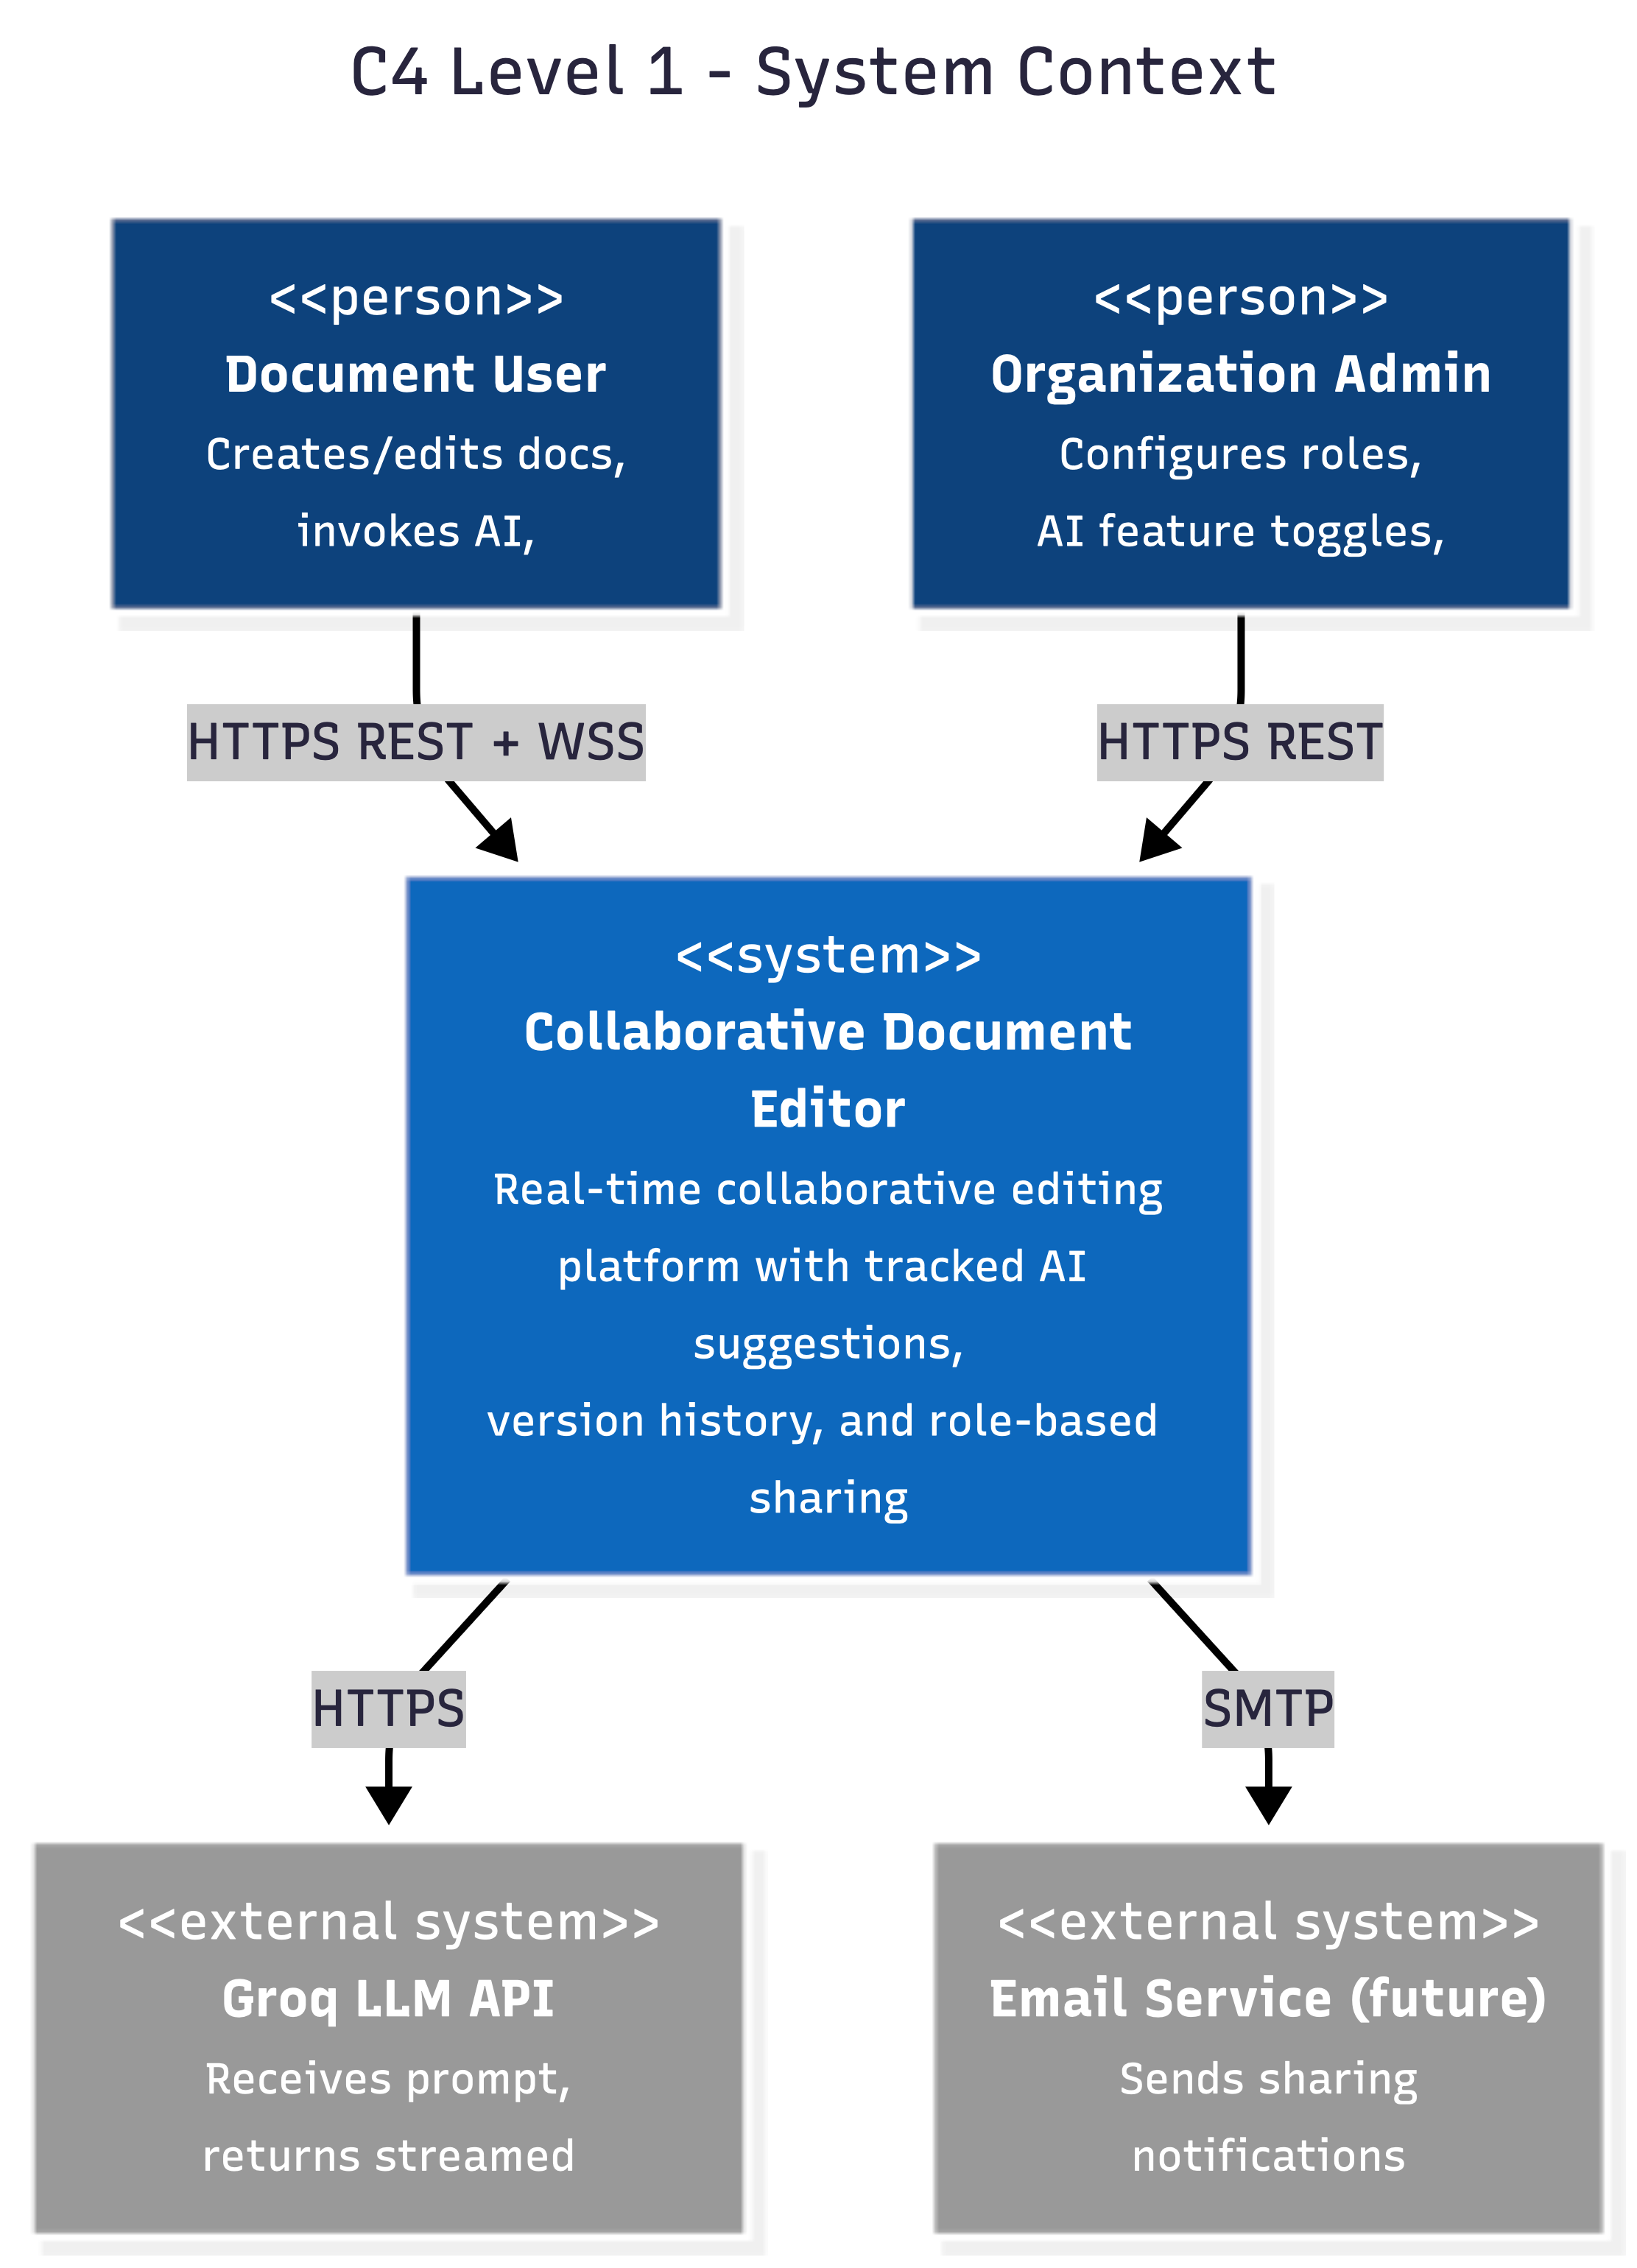
\includegraphics[width=0.55\textwidth]{docs/master_contract/diagrams/c4-context.png}
\end{center}

\vspace{5pt}
The current system boundary contains one product used by two human actor types. Document users interact with the editor, the AI assistant, and sharing/versioning functions. A separate organization-admin capability exists for AI policy configuration. The platform depends on Groq for inference and reserves an email integration for future sharing notifications.

\textbf{Level 2 - Container Diagram}

\begin{center}
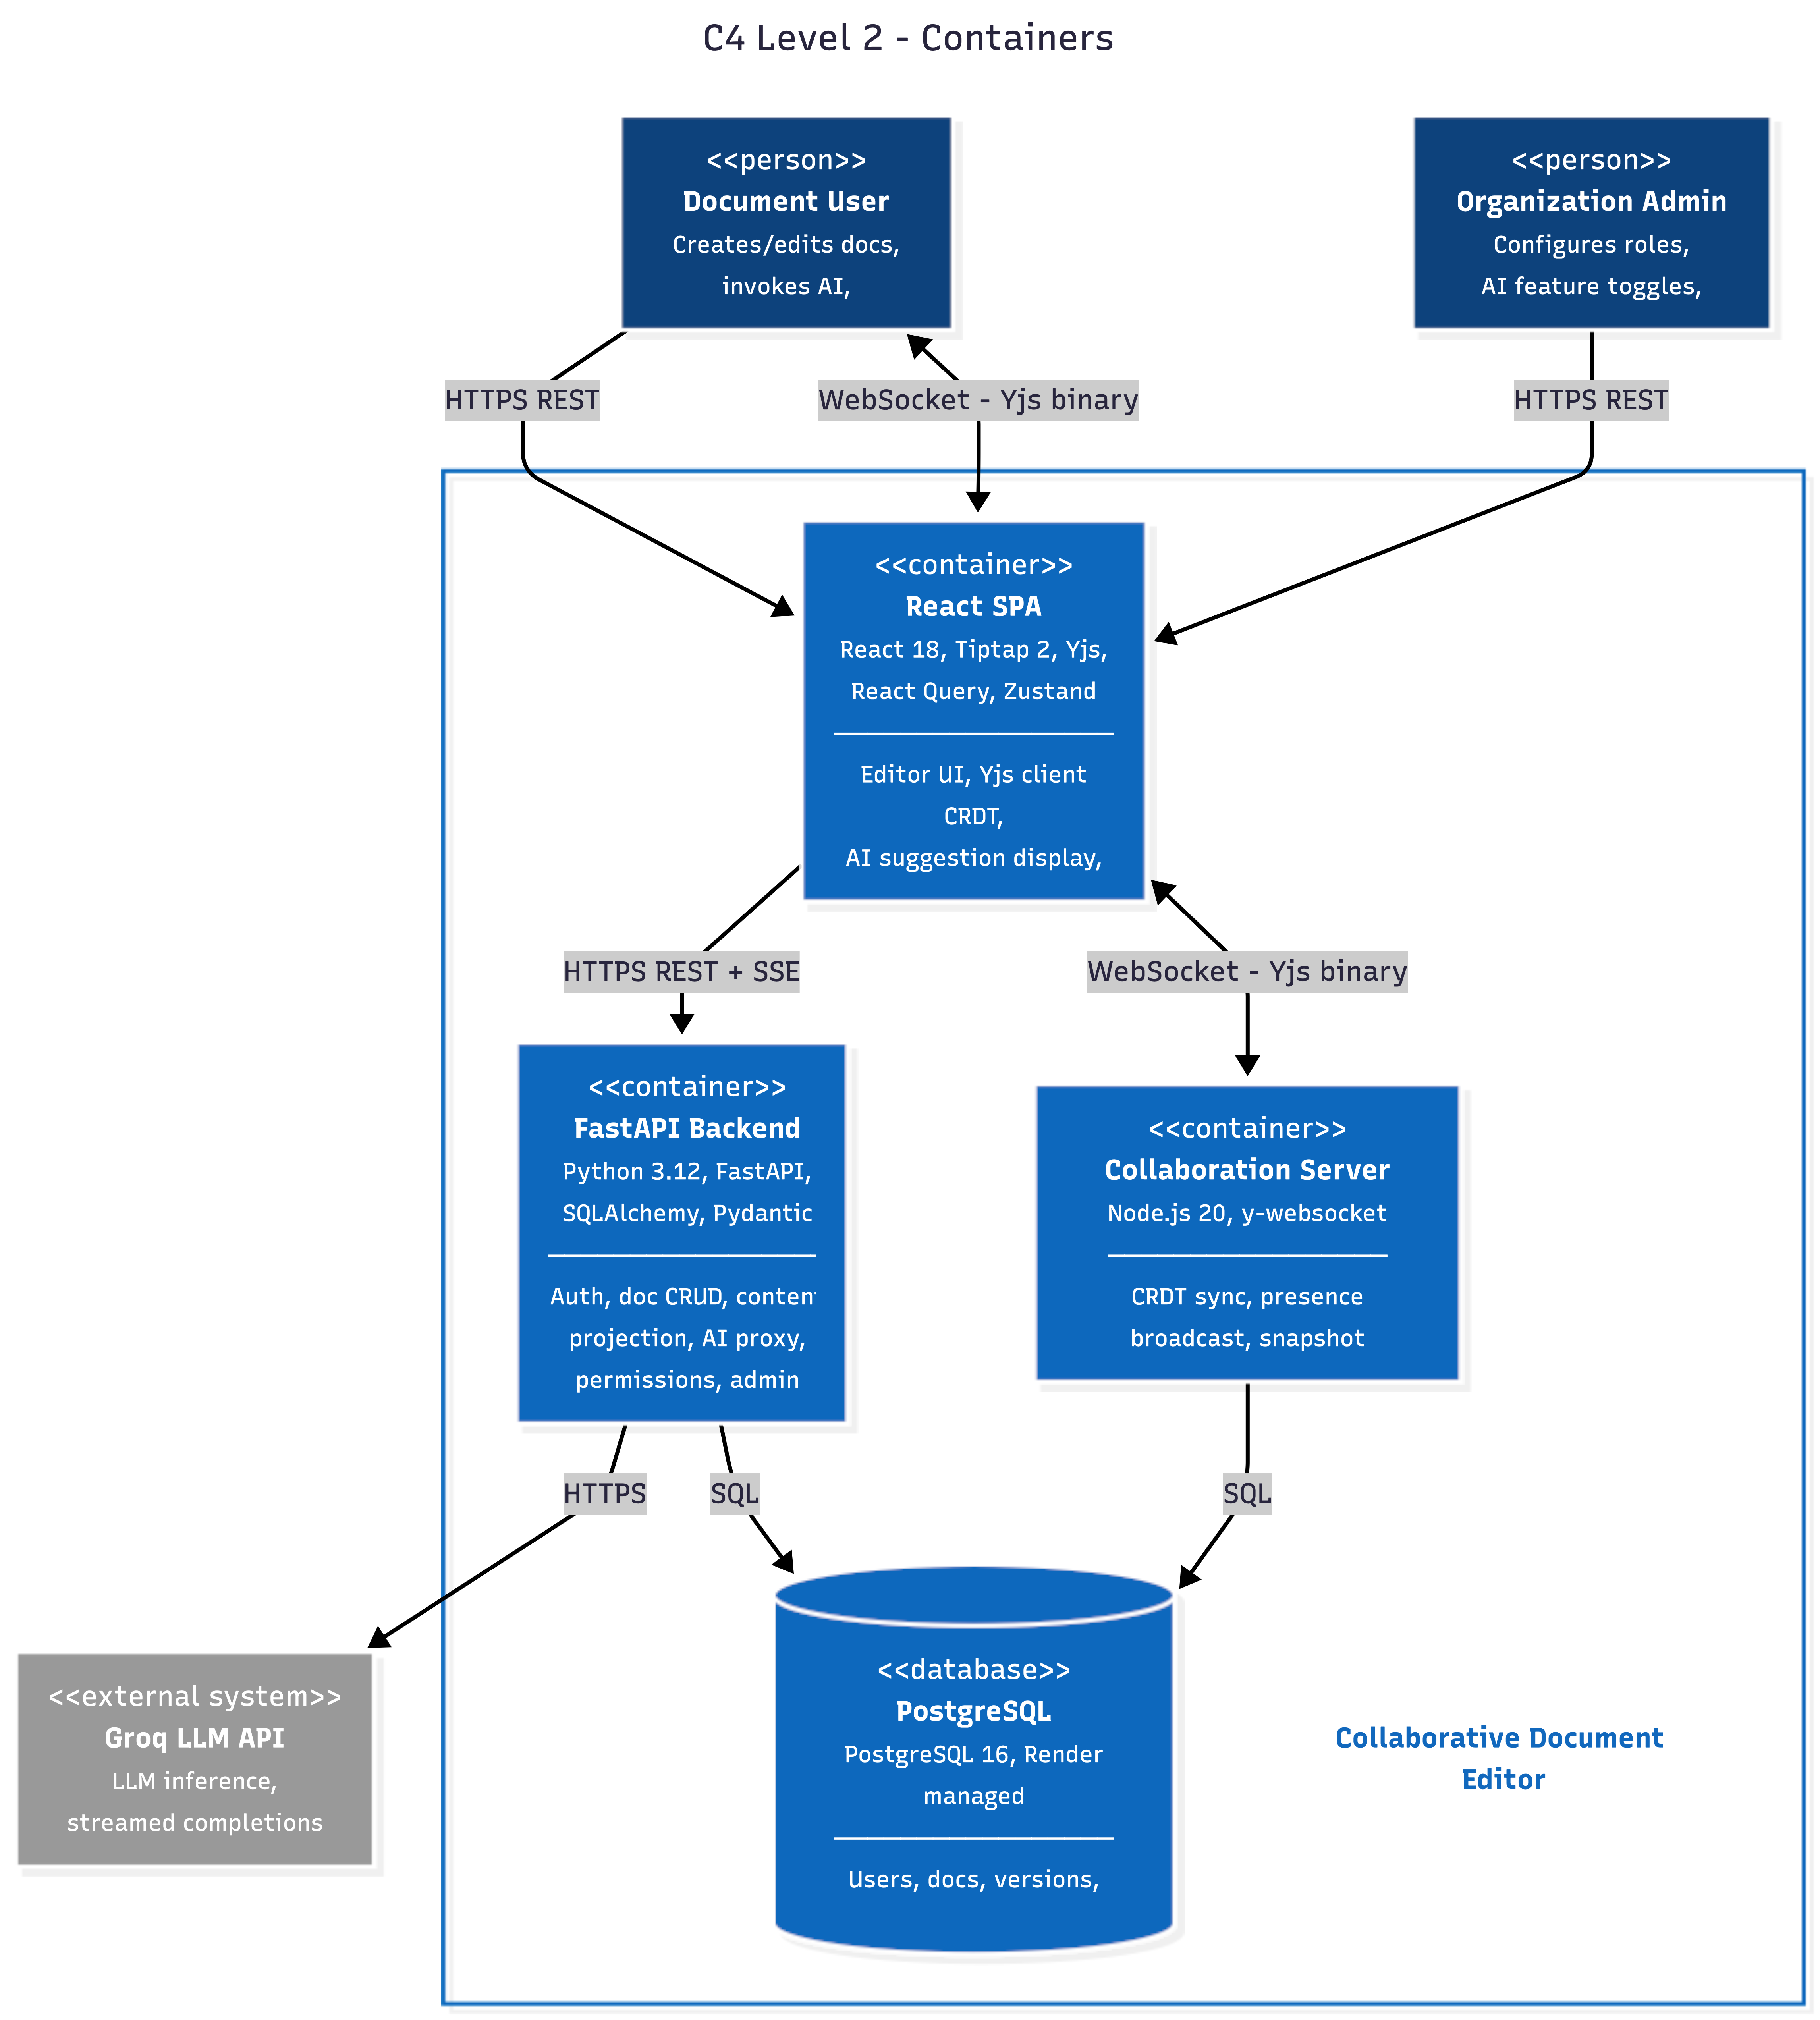
\includegraphics[width=0.82\textwidth]{docs/master_contract/diagrams/c4-container.png}
\end{center}

\vspace{5pt}
The current deployed system has four runtime containers. The browser talks to FastAPI for document, auth, permission, admin, and AI flows, and connects directly to the \texttt{y-websocket} service for rich-editor collaboration. PostgreSQL is shared by both services. The backend also maintains a strict REST document-content projection so the editor, export, and AI apply flows can reload authoritative text content while the collaboration server persists Yjs snapshots independently.

\textbf{Level 3 - Component Diagram}

\begin{center}
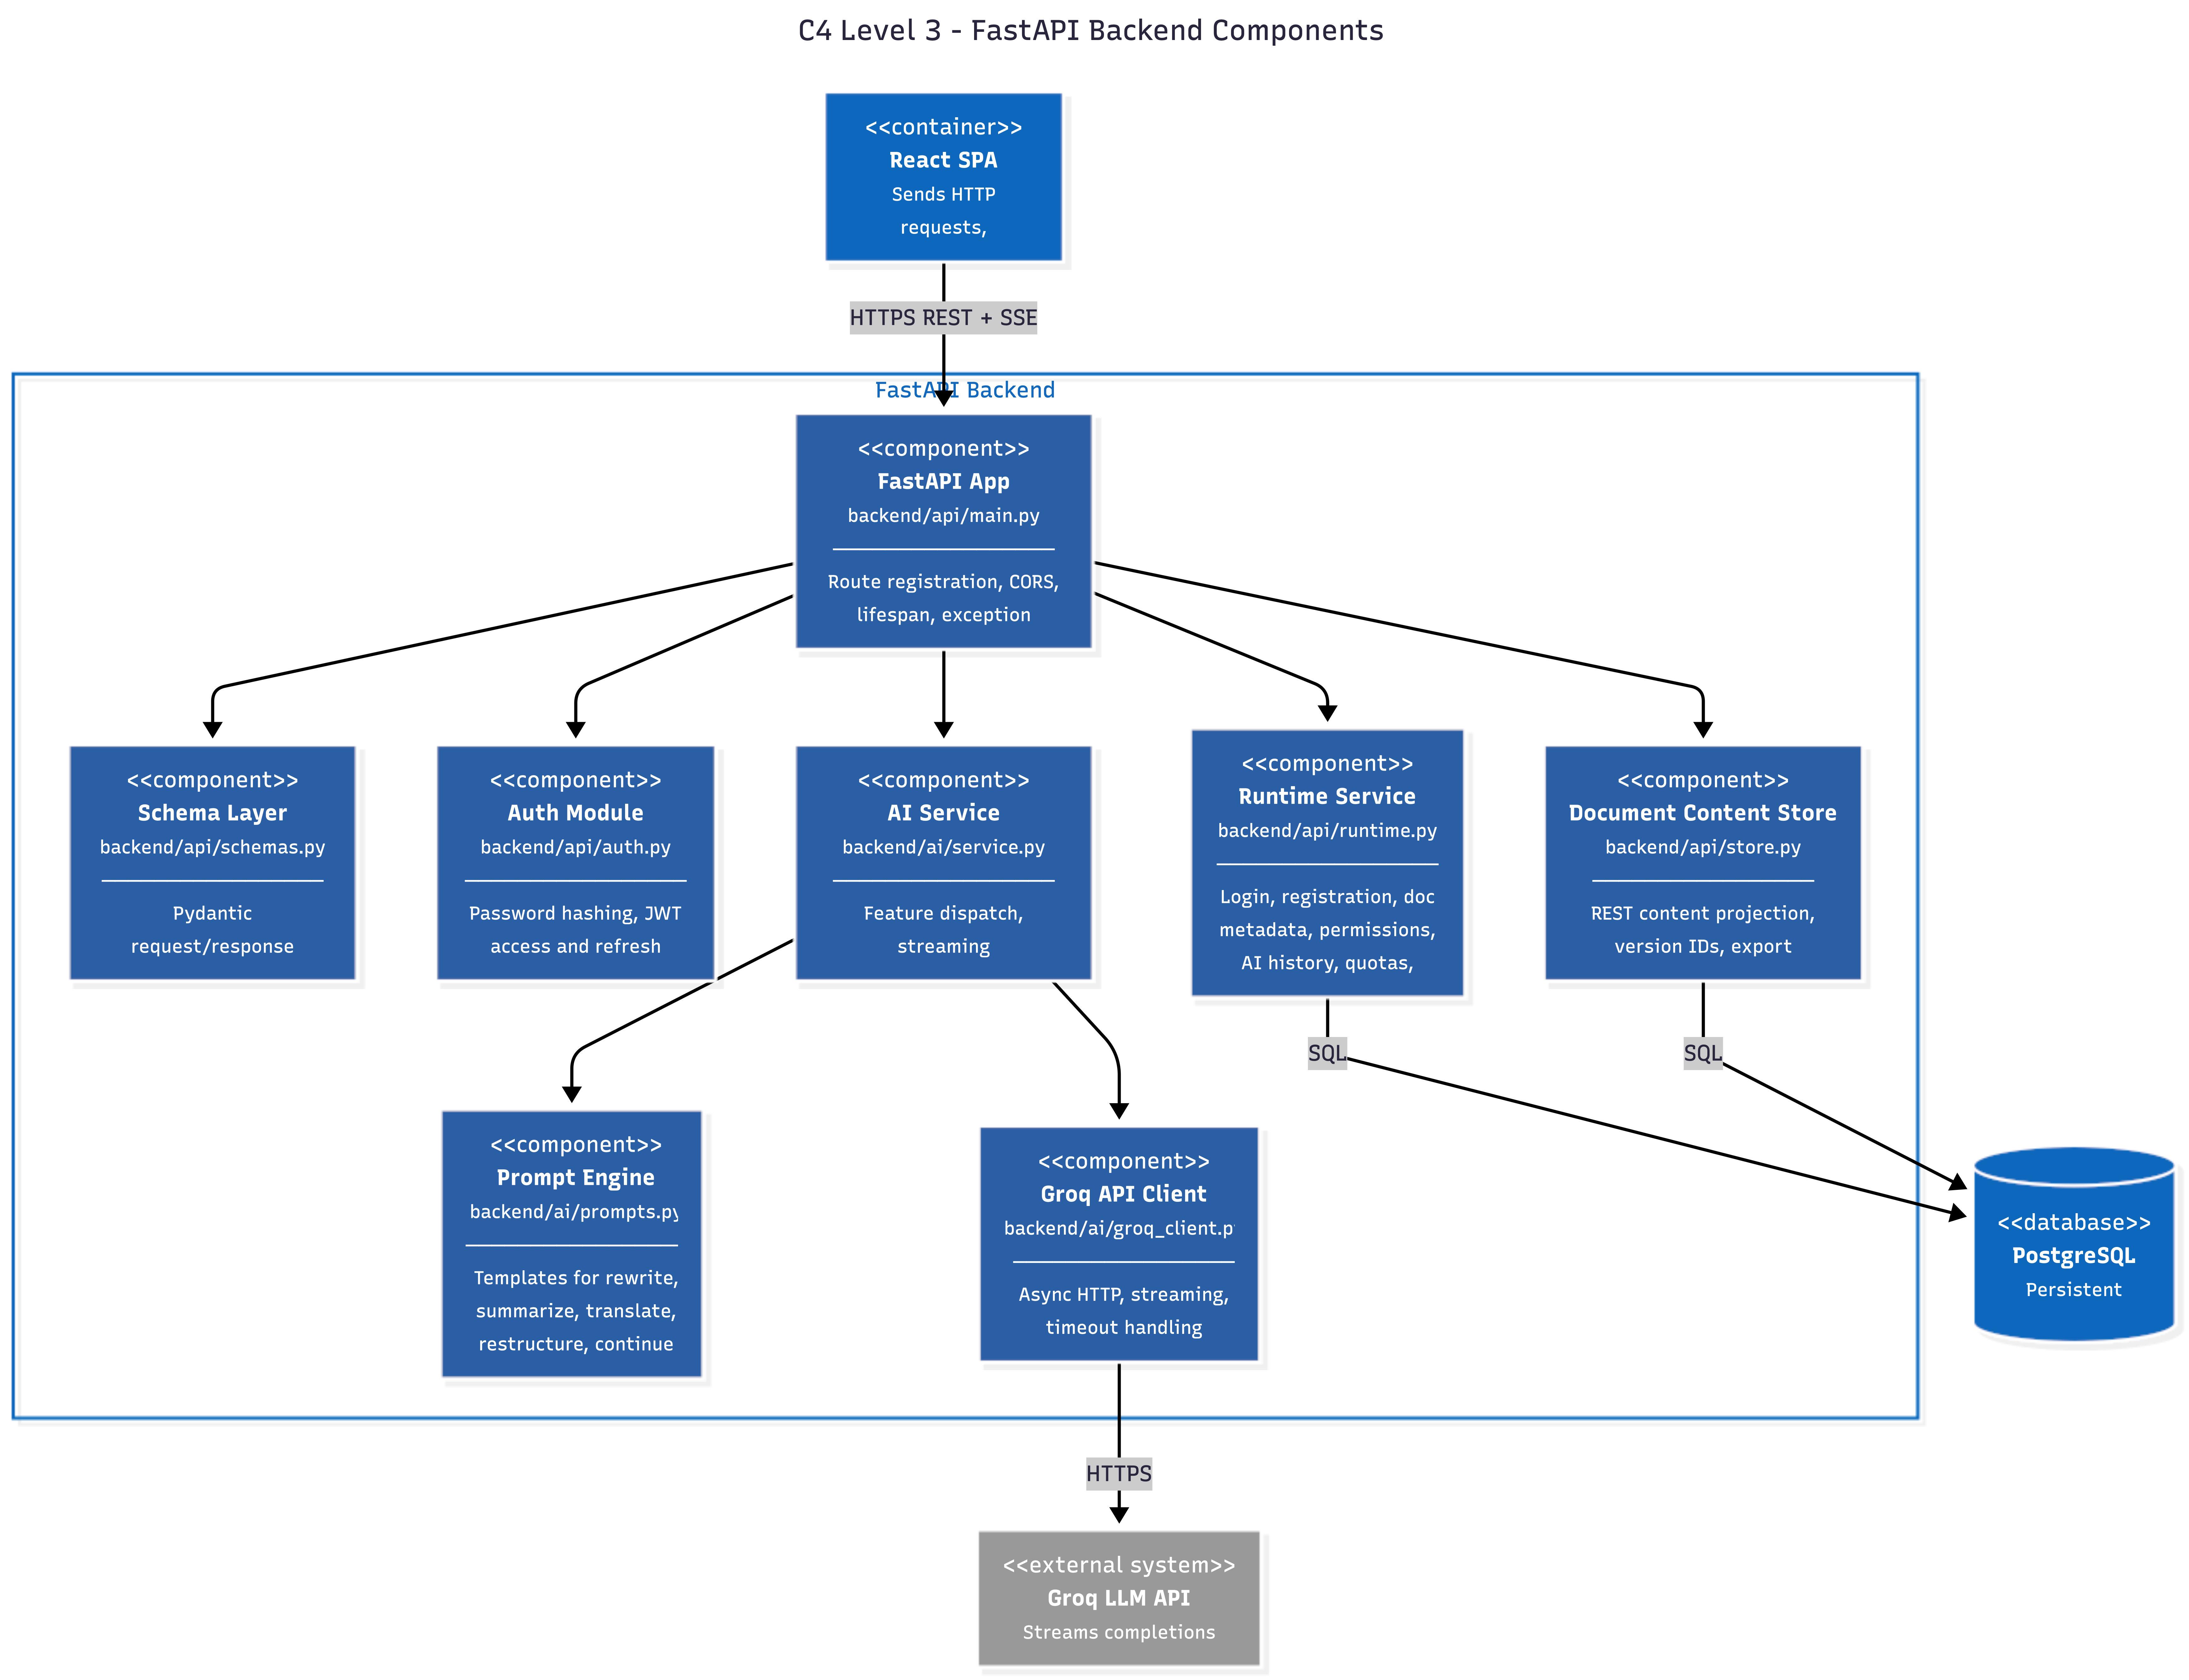
\includegraphics[width=\textwidth]{docs/master_contract/diagrams/c4-component-backend.png}
\end{center}

\vspace{5pt}
This component view reflects the code as it exists today, not a future refactor. \texttt{main.py} still owns route registration and request orchestration. \texttt{auth.py} handles password hashing and JWTs, \texttt{runtime.py} centralizes most metadata and permission logic, \texttt{store.py} owns the strict REST document-content projection, and \texttt{backend/ai/*} owns prompt construction plus Groq streaming.































\subsubsection{Feature Decomposition}
\noindent The current proof-of-concept is organized into six practical modules that line up with the shipped codebase.

\vspace{5pt}
\noindent\textbf{Rich-text editor and frontend state management.} The frontend now exposes a single editing surface: \texttt{ExperimentalTiptapEditor}, the live-sync rich editor backed by Yjs. \texttt{App.tsx} coordinates authentication, document loading, AI invocation, and apply/reject flows. Client state is split between hook-local state (\texttt{useAuth}, \texttt{useDocument}, \texttt{useAI}, \texttt{useVersionConflict}) and a single Zustand store, \texttt{editorStore}, which tracks realtime connection status, active session metadata, and presence count. \texttt{useRealtimeSession} is the only part already wired through React Query.

\vspace{5pt}
\noindent\textbf{Real-time synchronisation layer.} Rich-mode collaboration uses a \texttt{Y.Doc}, a \texttt{WebsocketProvider}, and Tiptap collaboration extensions from \texttt{frontend/src/extensions/realtimeEditor.ts}. The browser first calls \texttt{POST /api/realtime/session} to obtain a role-scoped WSS URL and awareness identity. The Node-based collaboration server in \texttt{backend/collab/server.js} handles Yjs update propagation and awareness broadcasts. \texttt{backend/collab/persistence.js} restores and persists Yjs snapshots when PostgreSQL is configured, and falls back to ephemeral mode when it is not.

\vspace{5pt}
\noindent\textbf{AI assistant service.} The current AI path is implemented in \texttt{backend/ai/service.py}, \texttt{backend/ai/prompts.py}, \texttt{backend/ai/groq\_client.py}, and \texttt{backend/ai/quota.py}. On the frontend, \texttt{AISidebar} and \texttt{useAI} drive rewrite, summarize, translate, restructure, and continue-writing requests. The shipped user experience is preview-first: the response streams into the sidebar, can be cancelled, and can be applied or rejected. In the rich editor, that preview is also rendered inline during review. This is less ambitious than a true shared tracked-change CRDT mark model, but it is the current code path.

\vspace{5pt}
\noindent\textbf{Document storage and versioning.} The implementation currently uses a strict REST document-content projection plus the rich-editor snapshot history. \texttt{backend/api/store.py} persists the reloadable text projection and version numbers via \texttt{document\_live\_content} and \texttt{document\_text\_versions}. In parallel, the collaboration server writes Yjs snapshots into \texttt{document\_versions}. Metadata, permissions, and ownership remain in \texttt{documents} and \texttt{permissions}.

\vspace{5pt}
\noindent\textbf{User authentication and authorization.} Authentication is stateless and JWT-based. \texttt{backend/api/auth.py} handles password hashing and token issue/validation, while \texttt{backend/api/runtime.py} manages registration, login, preview-user bootstrapping, per-document role resolution, and singleton organization-admin AI settings. The document roles enforced by the current code are \texttt{owner}, \texttt{editor}, \texttt{commenter}, and \texttt{viewer}.

\vspace{5pt}
\noindent\textbf{API layer.} The FastAPI app in \texttt{backend/api/main.py} owns request routing, error mapping, and application lifecycle. It exposes auth, strict document CRUD, permissions, realtime bootstrap, AI streaming and feedback, AI history deletion, and admin policy routes. Pydantic schemas in \texttt{backend/api/schemas.py} define the live request and response contracts consumed by the frontend.

\hspace{1cm}


\textbf{Role-Permission Matrix}


\noindent
{\small
\begin{tabularx}{\textwidth}{|>{\hsize=1\hsize\raggedright\arraybackslash}X|>{\hsize=1\hsize\raggedright\arraybackslash}X|>{\hsize=1\hsize\raggedright\arraybackslash}X|>{\hsize=1\hsize\raggedright\arraybackslash}X|>{\hsize=1\hsize\raggedright\arraybackslash}X|}
    \hline
    \rowcolor{tableBlue}
    \textbf{\color{white}Action} &
    \textbf{\color{white}Owner} &
    \textbf{\color{white}Editor} &
    \textbf{\color{white}Commenter} &
    \textbf{\color{white}Viewer} \\
    \hline
    View document & $\checkmark$ & \checkmark & \checkmark & \checkmark \\
    \hline
    Edit content & $\checkmark$ & \checkmark & $\times$ & $\times$ \\
    \hline
    Add comments & \checkmark & \checkmark & \checkmark & $\times$ \\
    \hline
    Invoke AI & \checkmark & \checkmark & $\times$ & $\times$ \\
    \hline
    Accept / reject AI & \checkmark & \checkmark & $\times$ & $\times$ \\
    \hline
    View version history & \checkmark & \checkmark & \checkmark & $\times$ \\
    \hline
    Revert to version & \checkmark & \checkmark & $\times$ & $\times$ \\
    \hline
    Share / manage permissions & \checkmark & $\times$ & $\times$ & $\times$ \\
    \hline
    Delete document & \checkmark & $\times$ & $\times$ & $\times$ \\
    \hline
    Export & \checkmark & \checkmark & \checkmark & \checkmark \\
    \hline
    Configure AI& \multicolumn{4}{c|}{Original Admin only} \\
    \hline
\end{tabularx}
}

\vspace{5pt}
\noindent\textbf{API Layer.} The API layer connects the React SPA to all backend services through a structured set of REST endpoints implemented in FastAPI. It is responsible for request routing, input validation via Pydantic schemas, error normalization, and SSE stream management for AI responses. The API layer depends on the backend runtime, auth helpers, schemas, document-content store, and AI service. Frontend TypeScript types and backend Pydantic schemas are currently maintained in parallel, so contract consistency is enforced through tests and documentation rather than generated shared packages.
\newpage
\textbf{Decided Technology Stack}


\noindent
{\small
\begin{tabularx}{\textwidth}{|>{\hsize=0.4\hsize\raggedright\arraybackslash}X|>{\hsize=0.5\hsize\raggedright\arraybackslash}X|>{\hsize=1.1\hsize\raggedright\arraybackslash}X|}
    \hline
    \rowcolor{tableBlue}
    \textbf{\color{white}Layer} &
    \textbf{\color{white}Technology} &
    \textbf{\color{white}Justification} \\
    \hline
    Frontend Framework & React 18 & Team familiarity; largest ecosystem; first-class Tiptap integration. \\
    \hline
    Rich Text Editor & Tiptap 2 (ProseMirror) & Already integrated in the current codebase and wired to the Yjs collaboration extensions currently in use. \\
    \hline
    CRDT Library & Yjs 13 & Most mature JavaScript CRDT; built-in awareness for cursors and presence, offline support, and sub-document editing. Automerge rejected for weaker rich-text support; ShareDB rejected due to OT complexity and limited offline capability. \\
    \hline
    CRDT Sync Server & y-websocket & Reference Yjs synchronisation implementation; lightweight and well-tested. Known limitation: single-instance, no horizontal scaling. \\
    \hline
    Build Tool & Vite 5 & Fast HMR for React development; simpler configuration than Webpack. \\
    \hline
    Client State & Hook-local React state + Zustand 5 & The current code centralizes realtime collaboration metadata in \texttt{editorStore}, while auth, document, and AI state remain hook-local. \\
    \hline
    Server State & React Query (TanStack) 5 & Currently used for realtime session bootstrap and suitable for further REST caching as the frontend matures. \\
    \hline
    Backend Framework & FastAPI 0.116.1 & Async Python backend with native request validation and SSE support. \\
    \hline
    Database Driver & asyncpg & Direct async PostgreSQL access is what the current backend actually uses. \\
    \hline
    Validation & Pydantic v2 & Defines the live request and response contracts in \texttt{backend/api/schemas.py}. \\
    \hline
    Database & PostgreSQL 16 & Render-managed persistence for users, documents, document content projections, Yjs snapshots, permissions, and AI logs. \\
    \hline
    LLM API & Groq — llama-3.3-70b-versatile & Ultra-low latency via LPU hardware; cost-effective; fast time-to-first-token for streaming UX; input data not used for model training. \\
    \hline
    Authentication & JWT (PyJWT + bcrypt) & This is the library stack used by the current implementation in \texttt{backend/api/auth.py}. \\
    \hline
    Deployment & Render & Managed hosting with built-in TLS, managed PostgreSQL, and multi-service Blueprint deployment. \\
    \hline
    Repository & Monorepo (single Git repo) & Enables atomic cross-boundary commits, a single CI pipeline, and shared contracts maintained in parallel across a four-person team. \\
    \hline
\end{tabularx}
}














\subsubsection{AI Integration Design}

\noindent
{\small
\begin{tabularx}{\textwidth}{|>{\hsize=0.5\hsize\raggedright\arraybackslash}X|>{\hsize=0.7\hsize\raggedright\arraybackslash}X|>{\hsize=0.8\hsize\raggedright\arraybackslash}X|}
    \hline
    \rowcolor{tableBlue}
    \textbf{\color{white}Decision Area} &
    \textbf{\color{white}Decision} &
    \textbf{\color{white}Rationale} \\
    \hline
    Context transmitted to Groq & Rewrite, summarize, translate, and restructure requests are selection-scoped; continue-writing uses a recent trailing excerpt of the document. Full-document context is not sent by default. & Keeps prompts cheaper, faster, and less privacy-invasive while still giving the model enough local context to respond well. \\
    \hline
    Full-document summarisation & Not exposed in the current client. Summarisation operates on the active selection and is presented as a suggestion against that local scope. & Matches the current code and avoids claiming a long-document summarisation workflow the PoC does not yet ship. \\
    \hline
    Suggestion UX & The current PoC is preview-first. The sidebar streams the generated suggestion, and the user explicitly applies or rejects it. In rich mode the editor also renders a temporary inline preview surface during review. & Matches the code that is currently shipped, even though a deeper Yjs-native tracked-change model remains a future refinement. \\
    \hline
    AI during concurrent editing & Collaboration remains live during AI requests. The initiating client reviews the generated preview and then applies it through the normal document update path. The stricter soft-lock policy remains a documented future refinement rather than current shipped behavior. & Honest representation of the implemented behavior. The current PoC proves AI plus sync can coexist without yet claiming paragraph-level region locks. \\
    \hline
    Prompt storage & Prompt templates live in \texttt{backend/ai/prompts.py}, with per-feature helpers for rewrite, summarize, translate, restructure, and continue-writing. & Prompt updates remain isolated from route and UI code. \\
    \hline
    Model selection & \texttt{llama-3.3-70b-versatile} via Groq for all features; \texttt{llama-3.1-8b} available as a fallback for budget-constrained operations. & Strong output quality at low cost; Groq LPU hardware delivers fast first-token latency. \\
    \hline
    Cost control & Three-tier enforcement: (1) per-user daily quota of 50,000 tokens tracked in the database; (2) organisation-level monthly budget configurable by admins; (3) per-request input cap of 4,000 tokens with automatic truncation. & Layered defence against cost overrun; quota exhaustion returns HTTP 429 with a clear message. \\
    \hline
    Backend proxy & All AI requests are routed frontend $\rightarrow$ backend $\rightarrow$ Groq; direct frontend-to-Groq calls are not permitted. & Conceals the API key; guarantees server-side logging and quota enforcement; the additional network hop (~10--50\,ms) is acceptable. \\
    \hline
\end{tabularx}
}









\newpage
\subsubsection{API Design}
\vspace{5pt}
\noindent\textbf{Documents}
\vspace{5pt}

\noindent
{\small
\begin{tabularx}{\textwidth}{|>{\hsize=0.3\hsize\raggedright\arraybackslash}X|>{\hsize=0.85\hsize\raggedright\arraybackslash}X|>{\hsize=0.4\hsize\raggedright\arraybackslash}X|>{\hsize=0.45\hsize\raggedright\arraybackslash}X|}
    \hline
    \rowcolor{tableBlue}
    \textbf{\color{white}Method} &
    \textbf{\color{white}Endpoint} &
    \textbf{\color{white}Body / Parameters} &
    \textbf{\color{white}Response} \\
    \hline
    POST & \texttt{/api/documents} & \texttt{\{title\}} & \texttt{\{id, title, owner\_id, created\_at\}} \\
    \hline
    GET & \texttt{/api/documents} & — & \texttt{[\{id, title, role, updated\_at\}]} \\
    \hline
    GET & \texttt{/api/documents/:id} & — & \texttt{\{id, title, content, owner, permissions, updated\_at, version\_id\}} \\
    \hline
    PUT & \texttt{/api/documents/:id} & \texttt{\{content, versionId\}} & \texttt{\{id, title, content, versionId, lastModified\}} \\
    \hline
    PATCH & \texttt{/api/documents/:id} & \texttt{\{title\}} & \texttt{\{id, title, updated\_at\}} \\
    \hline
    DELETE & \texttt{/api/documents/:id} & — & \texttt{204} \\
    \hline
    POST & \texttt{/api/documents/:id/restore} & — & \texttt{\{id, title, updated\_at, restored\}} \\
    \hline
    POST & \texttt{/api/documents/:id/snapshot} & \texttt{\{snapshot: base64\}} & \texttt{\{version\_id, created\_at\}} \\
    \hline
    GET & \texttt{/api/documents/:id/versions} & — & \texttt{[\{version\_id, created\_at, created\_by\}]} \\
    \hline
    POST & \texttt{/api/documents/:id/revert/:vid} & — & \texttt{\{version\_id, created\_at\}} \\
    \hline
    GET & \texttt{/api/documents/:id/export?format=pdf|docx|md} & — & Binary download \\
    \hline
\end{tabularx}
}

\vspace{10pt}
\noindent\textbf{AI}
\vspace{5pt}

\noindent
{\small
\begin{tabularx}{\textwidth}{|>{\hsize=0.3\hsize\raggedright\arraybackslash}X|>{\hsize=0.7\hsize\raggedright\arraybackslash}X|>{\hsize=0.6\hsize\raggedright\arraybackslash}X|>{\hsize=0.4\hsize\raggedright\arraybackslash}X|}
    \hline
    \rowcolor{tableBlue}
    \textbf{\color{white}Method} &
    \textbf{\color{white}Endpoint} &
    \textbf{\color{white}Body} &
    \textbf{\color{white}Response} \\
    \hline
    POST & \texttt{/api/ai/rewrite} & \texttt{\{doc\_id, selection, (context), style?\}} & SSE stream: \texttt{\{token, done, suggestion\_id\}} \\
    \hline
    POST & \texttt{/api/ai/summarize} & \texttt{\{doc\_id, selection, context?\}} & SSE stream \\
    \hline
    POST & \texttt{/api/ai/translate} & \texttt{\{doc\_id, selection, (context), target\_lang\}} & SSE stream \\
    \hline
    POST & \texttt{/api/ai/restructure} & \texttt{\{doc\_id, selection, (context), instructions\}} & SSE stream \\
    \hline
    POST & \texttt{/api/ai/continue} & \texttt{\{doc\_id, selection, notes?\}} & SSE stream \\
    \hline
    POST & \texttt{/api/ai/cancel/:suggestion\_id} & — & \texttt{200} \\
    \hline
    POST & \texttt{/api/ai/feedback} & \texttt{\{suggestion\_id, action\}} & \texttt{200} \\
    \hline
    GET & \texttt{/api/ai/history} & \texttt{?doc\_id=\&limit=\&feature=\&status=} & \texttt{[\{id, feature, status, tokens\_used\}]} \\
    \hline
    DELETE & \texttt{/api/ai/history/:id} & — & \texttt{204} \\
    \hline
\end{tabularx}
}

\vspace{10pt}
\noindent\textbf{Error Codes}
\vspace{5pt}

\noindent
{\small
\begin{tabularx}{\textwidth}{|>{\hsize=0.3\hsize\raggedright\arraybackslash}X|>{\hsize=0.6\hsize\raggedright\arraybackslash}X|>{\hsize=1.1\hsize\raggedright\arraybackslash}X|}
    \hline
    \rowcolor{tableBlue}
    \textbf{\color{white}Status} &
    \textbf{\color{white}Code} &
    \textbf{\color{white}When} \\
    \hline
    400 & \texttt{INVALID\_REQUEST} & Malformed request body or missing required fields. \\
    \hline
    401 & \texttt{TOKEN\_EXPIRED} & JWT has expired; client should attempt a token refresh. \\
    \hline
    403 & \texttt{INSUFFICIENT\_PERMISSION} & The requesting role does not permit the attempted action. \\
    \hline
    404 & \texttt{DOCUMENT\_NOT\_FOUND} & Document does not exist or the requesting user has no access. \\
    \hline
    429 & \texttt{AI\_QUOTA\_EXCEEDED} & The user's daily AI token limit has been reached. \\
    \hline
    503 & \texttt{AI\_SERVICE\_UNAVAILABLE} & Groq API is unreachable. \\
    \hline
    504 & \texttt{AI\_TIMEOUT} & Groq did not respond within the 30-second timeout window. \\
    \hline
\end{tabularx}
}








\vspace{10pt}


\subsubsection{Authentication \& Authorization}
\vspace{5pt}

\noindent
{\small
\begin{tabularx}{\textwidth}{|>{\hsize=0.3\hsize\raggedright\arraybackslash}X|>{\hsize=0.6\hsize\raggedright\arraybackslash}X|>{\hsize=0.5\hsize\raggedright\arraybackslash}X|>{\hsize=0.6\hsize\raggedright\arraybackslash}X|}
    \hline
    \rowcolor{tableBlue}
    \textbf{\color{white}Method} &
    \textbf{\color{white}Endpoint} &
    \textbf{\color{white}Body} &
    \textbf{\color{white}Response} \\
    \hline
    POST & \texttt{/api/auth/register} & \texttt{\{email, password, name\}} & \texttt{\{accessToken, refreshToken, user, expiresIn\}} \\
    \hline
    POST & \texttt{/api/auth/login} & \texttt{\{email, password\}} & \texttt{\{accessToken, refreshToken, user, expiresIn\}} \\
    \hline
    POST & \texttt{/api/auth/refresh} & \texttt{\{refreshToken\}} & \texttt{\{accessToken, refreshToken, user, expiresIn\}} \\
    \hline
    GET & \texttt{/api/users/me} & — & \texttt{\{id, email, name, role\}} \\
    \hline
\end{tabularx}
}

\vspace{10pt}
\noindent\textbf{Admin}
\vspace{5pt}

\noindent
{\small
\begin{tabularx}{\textwidth}{|>{\hsize=0.3\hsize\raggedright\arraybackslash}X|>{\hsize=0.6\hsize\raggedright\arraybackslash}X|>{\hsize=0.6\hsize\raggedright\arraybackslash}X|>{\hsize=0.9\hsize\raggedright\arraybackslash}X|}
    \hline
    \rowcolor{tableBlue}
    \textbf{\color{white}Method} &
    \textbf{\color{white}Endpoint} &
    \textbf{\color{white}Body} &
    \textbf{\color{white}Response} \\
    \hline
    GET & \texttt{/api/admin/ai-settings} & — & \texttt{\{feature\_access, daily\_token\_limit, monthly\_org\_token\_budget, consent\_required\}} \\
    \hline
    PATCH & \texttt{/api/admin/ai-settings} & \texttt{\{feature\_access?, daily\_token\_limit?, monthly\_org\_token\_budget?, consent\_required?\}} & \texttt{\{feature\_access, daily\_token\_limit, monthly\_org\_token\_budget, consent\_required\}} \\
    \hline
\end{tabularx}
}

\vspace{10pt}
\noindent\textbf{Permissions}
\vspace{5pt}

\noindent
{\small
\begin{tabularx}{\textwidth}{|>{\hsize=0.3\hsize\raggedright\arraybackslash}X|>{\hsize=0.7\hsize\raggedright\arraybackslash}X|>{\hsize=0.4\hsize\raggedright\arraybackslash}X|>{\hsize=0.6\hsize\raggedright\arraybackslash}X|}
    \hline
    \rowcolor{tableBlue}
    \textbf{\color{white}Method} &
    \textbf{\color{white}Endpoint} &
    \textbf{\color{white}Body} &
    \textbf{\color{white}Response} \\
    \hline
    POST & \texttt{/api/documents/:id/permissions} & \texttt{\{user\_email, role\}} & \texttt{\{permission\_id, user\_id, role\}} \\
    \hline
    GET & \texttt{/api/documents/:id/permissions} & — & \texttt{[\{user\_id, email, name, role\}]} \\
    \hline
    PATCH & \texttt{/api/documents/:id/permissions/:pid} & \texttt{\{role\}} & \texttt{\{permission\_id, role\}} \\
    \hline
    DELETE & \texttt{/api/documents/:id/permissions/:pid} & — & \texttt{204} \\
    \hline
\end{tabularx}
}


\textbf{Communication model}

\noindent
{\small
\begin{tabularx}{\textwidth}{|>{\hsize=0.5\hsize\raggedright\arraybackslash}X|>{\hsize=1\hsize\raggedright\arraybackslash}X|>{\hsize=0.7\hsize\raggedright\arraybackslash}X|>{\hsize=1.8\hsize\raggedright\arraybackslash}X|}
    \hline
    \rowcolor{tableBlue}
    \textbf{\color{white}Interaction} &
    \textbf{\color{white}Protocol} &
    \textbf{\color{white}Direction} &
    \textbf{\color{white}Justification} \\
    \hline
    Document CRUD & REST (HTTPS) & SPA $\rightarrow$ API & Simple, cacheable, and stateless; appropriate for request-response document operations. \\
    \hline
    Authentication & REST + JWT & SPA $\rightarrow$ API & Standard stateless authentication pattern for single-page applications. \\
    \hline
    AI invocation & REST + SSE streaming & SPA $\rightarrow$ API $\rightarrow$ Groq & SSE enables word-by-word delivery of AI responses, providing immediate user feedback without polling. \\
    \hline
    Real-time edits & WebSocket (Yjs binary protocol) & SPA $\leftrightarrow$ Collab Server & Low-latency bidirectional channel used only by the rich-editor collaboration path. \\
    \hline
    Presence (cursors) & WebSocket (Yjs Awareness) & SPA $\leftrightarrow$ Collab Server & Native Yjs awareness is already used to surface peer count and live editor state. \\
    \hline
    Snapshot persistence & SQL (internal) & Collab Server $\rightarrow$ DB & Yjs snapshots are restored and persisted by the collab server independently of the REST document-content projection. \\
    \hline
\end{tabularx}
}












\subsection{Code Structure \& Repository Organization}
\begin{footnotesize}
\begin{verbatim}
collab-editor/
|-- frontend/
|   |-- src/
|   |   |-- api/                     authAPI, documentAPI, mockAPI, realtimeAPI
|   |   |-- components/              App shell, rich editor, AI sidebar, auth and error UI
|   |   |-- extensions/              realtimeEditor.ts
|   |   |-- hooks/                   useAuth, useDocument, useAI, useRealtimeSession, useVersionConflict
|   |   |-- stores/                  editorStore.ts
|   |   |-- styles/                  shared CSS entrypoints
|   |   |-- types/                   frontend request and domain types
|   |   |-- App.tsx
|   |   `-- main.tsx
|   |-- tests/e2e/                   Playwright smoke test
|   |-- package.json
|   `-- vite.config.ts
|-- backend/
|   |-- api/
|   |   |-- auth.py                  JWT and password helpers
|   |   |-- config.py                environment-backed settings
|   |   |-- main.py                  FastAPI app and route surface
|   |   |-- runtime.py               user, document metadata, permission, quota, and admin policy logic
|   |   |-- schemas.py               Pydantic request and response models
|   |   `-- store.py                 strict document content projection and export path
|   |-- ai/
|   |   |-- groq_client.py           Groq API wrapper and streaming handler
|   |   |-- prompts.py               feature-specific prompt templates
|   |   |-- quota.py                 token estimation and quota helpers
|   |   `-- service.py               AI orchestration
|   |-- collab/
|   |   |-- server.js                y-websocket server entry point
|   |   `-- persistence.js           PostgreSQL snapshot adapter
|   |-- tests/
|   |   `-- test_api.py              backend integration-style tests
|   `-- requirements.txt
|-- docs/
|   |-- brief.md
|   |-- contract.md
|   |-- master_contract/
|   `-- submission/
|-- infra/
|   |-- init.sql
|   |-- render.yaml
|   `-- .env.example
`-- .github/workflows/               CI pipeline definitions
\end{verbatim}
\end{footnotesize}

\noindent The repository is a monorepo, but it is not yet split into a generated \texttt{shared/} contract package. Frontend TypeScript types and backend Pydantic schemas are still maintained in parallel. Configuration lives in \texttt{.env.example}, \texttt{frontend/.env.example}, and Render environment variables. Tests currently live under \texttt{backend/tests}, while frontend verification is handled through linting, builds, and a committed Playwright smoke test under \texttt{frontend/tests/e2e}.

\newpage
\subsection{Data Model}

\begin{center}
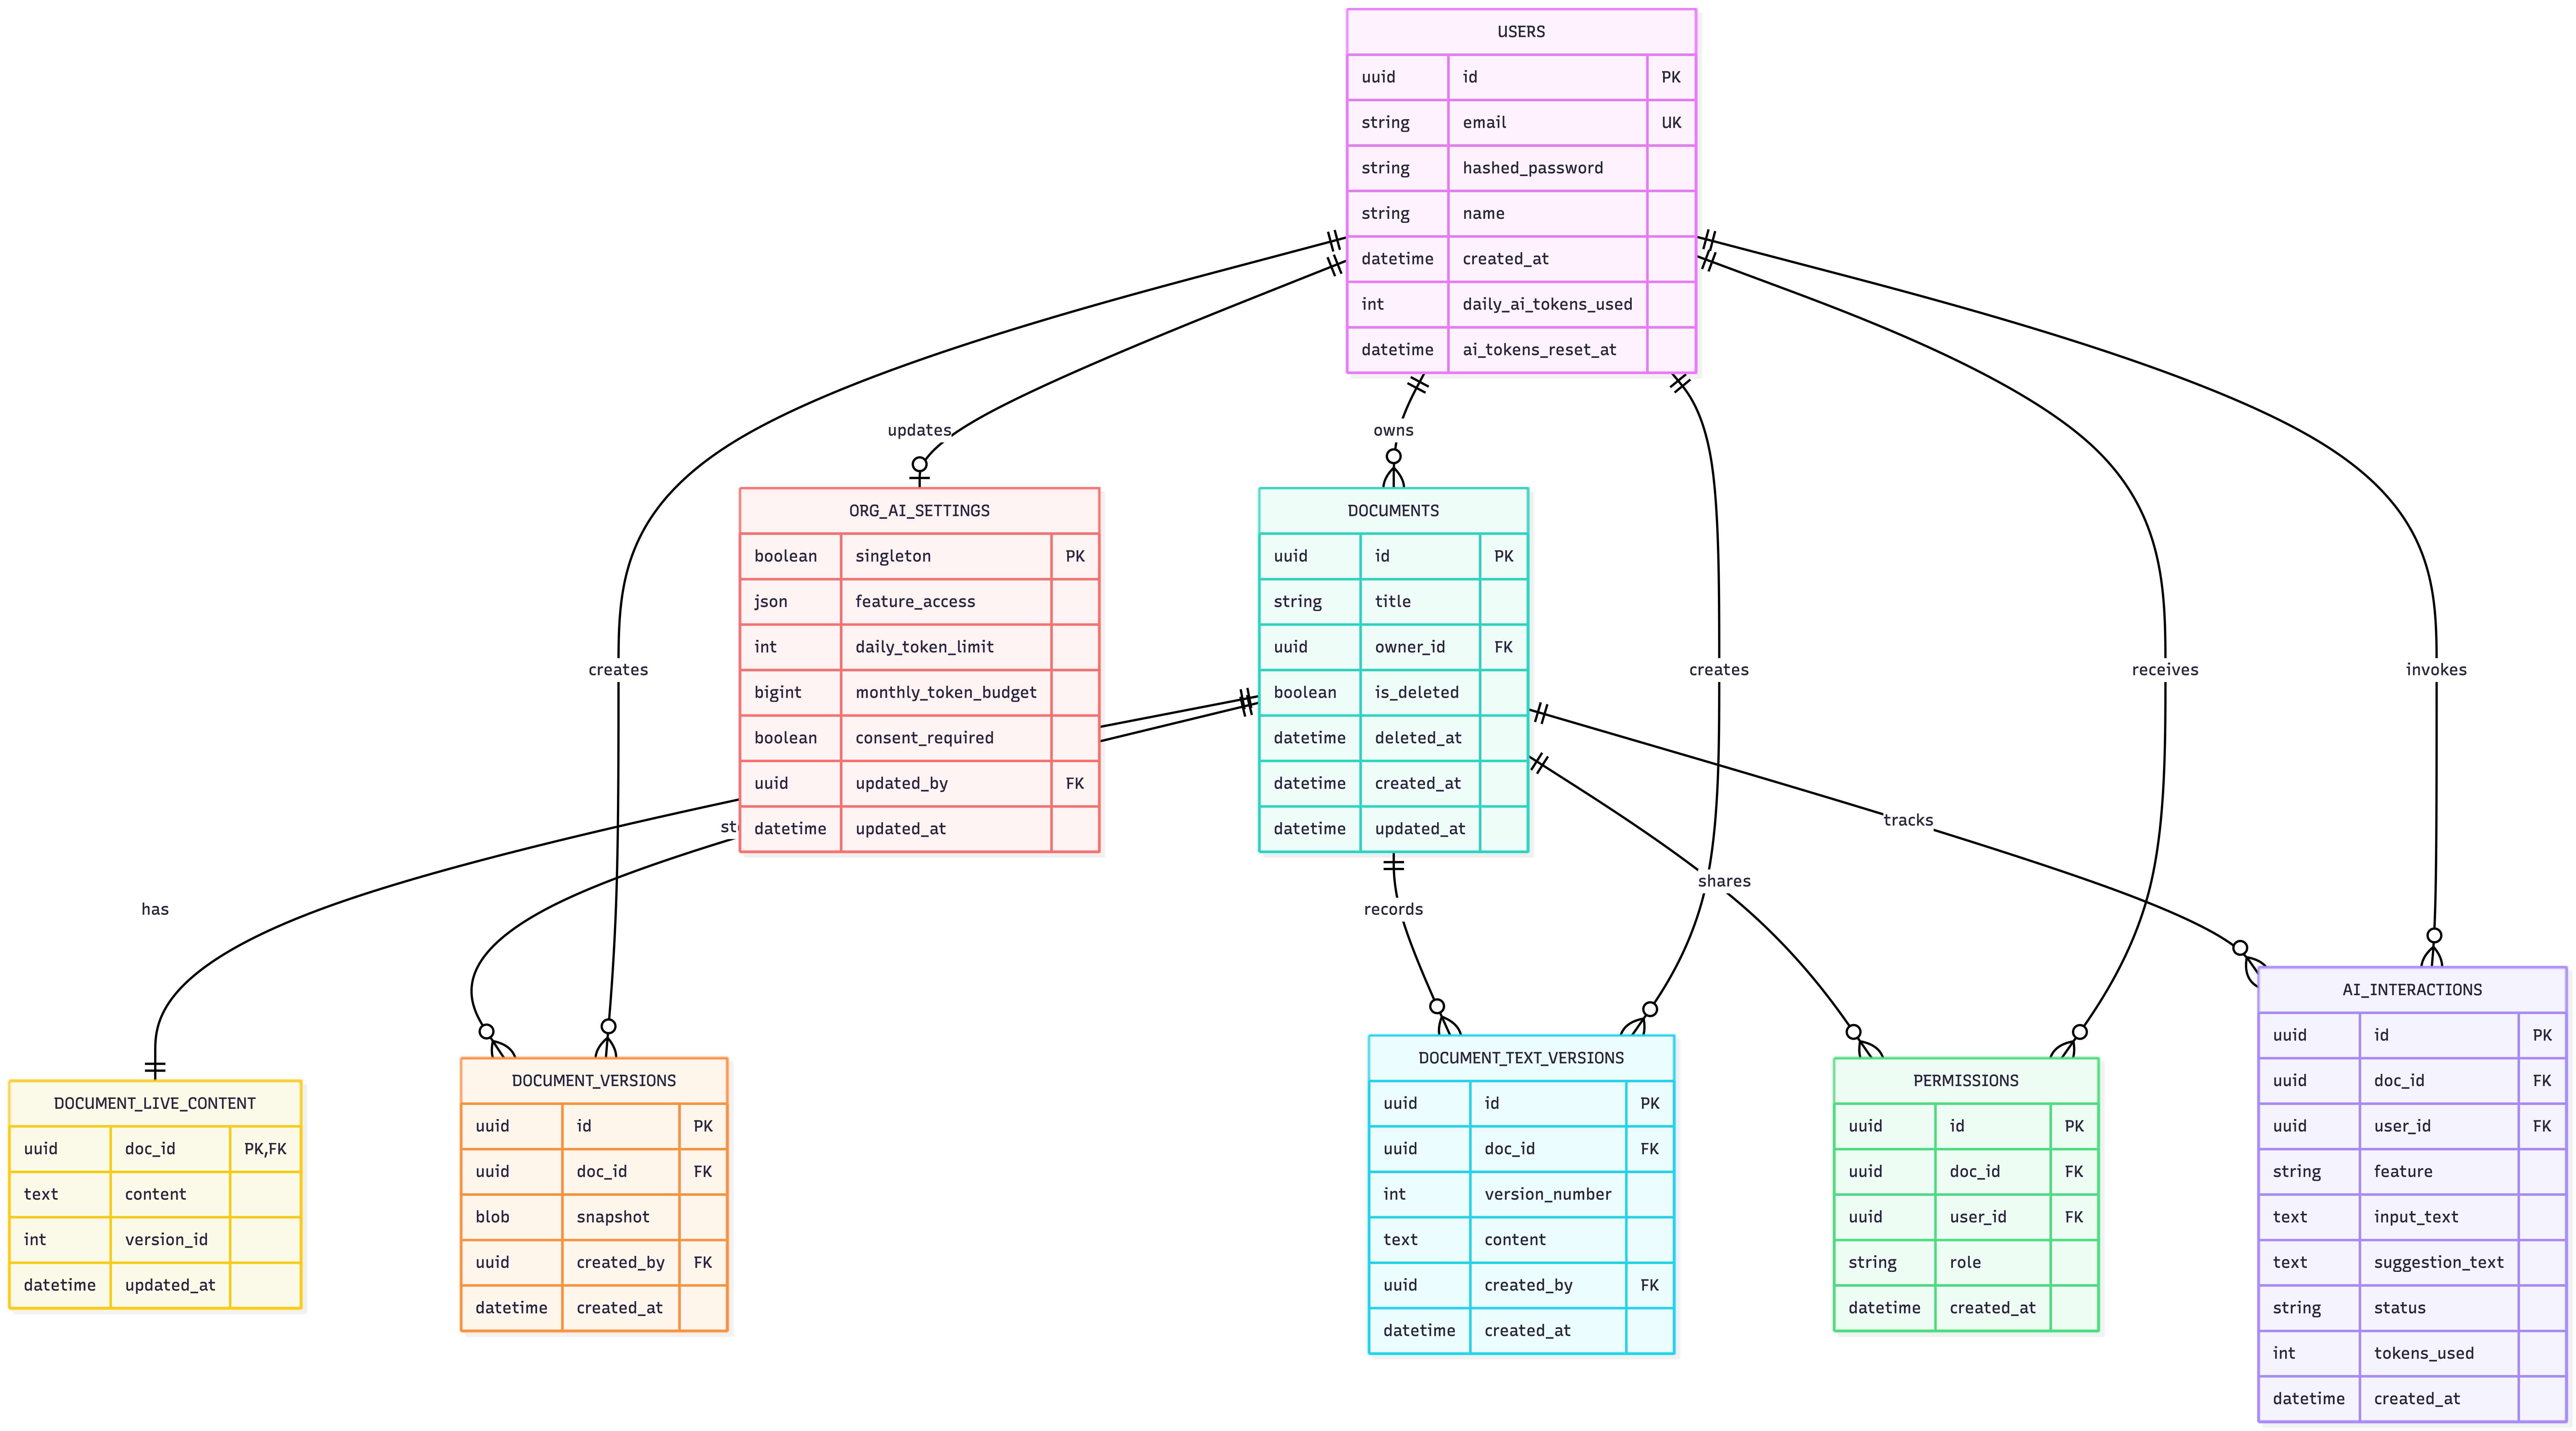
\includegraphics[width=\textwidth]{docs/master_contract/diagrams/erd.png}
\end{center}
\noindent
{\small
\begin{tabularx}{\textwidth}{|>{\hsize=0.5\hsize\raggedright\arraybackslash}X|>{\hsize=1\hsize\raggedright\arraybackslash}X|>{\hsize=1.5\hsize\raggedright\arraybackslash}X|}
    \hline
    \rowcolor{tableBlue}
    \textbf{\color{white}Table} &
    \textbf{\color{white}Key Columns} &
    \textbf{\color{white}Design Notes} \\
    \hline
\texttt{users} &
\texttt{id} (UUID PK), \texttt{email} (unique), \texttt{hashed\_password}, \texttt{name}, \texttt{created\_at}, \texttt{daily\_ai\_tokens\_used}, \texttt{ai\_tokens\_reset\_at} &
Manages authentication credentials and per-user AI resource consumption. The daily token counter resets automatically when the current timestamp exceeds \texttt{ai\_tokens\_reset\_at}, allowing a lightweight quota cycle without scheduled jobs. \\
\hline
\texttt{documents} &
\texttt{id} (UUID PK), \texttt{title}, \texttt{owner\_id} (FK $\rightarrow$ users), \texttt{created\_at}, \texttt{updated\_at}, \texttt{is\_deleted}, \texttt{deleted\_at} &
Stores document metadata and soft-delete state. \texttt{owner\_id} is also stored here for fast ownership lookups, in addition to the entry in \texttt{permissions}. \\
\hline
\texttt{document\_live\_content} &
\texttt{doc\_id} (UUID PK/FK), \texttt{content}, \texttt{version\_id}, \texttt{updated\_at} &
Stores the reloadable REST document-content projection exposed through \texttt{/api/documents/:id}. This is what the frontend reloads after AI apply, export, and version checks. \\
\hline
\texttt{document\_text\_versions} &
\texttt{id} (UUID PK), \texttt{doc\_id} (FK $\rightarrow$ documents), \texttt{version\_number}, \texttt{content}, \texttt{created\_by} (FK $\rightarrow$ users), \texttt{created\_at} &
Append-only text versions used for REST-side history, revert, export, and AI-apply auditing. \\
\hline
\texttt{document\_versions} &
\texttt{id} (UUID PK), \texttt{doc\_id} (FK $\rightarrow$ documents), \texttt{snapshot} (bytea), \texttt{created\_at}, \texttt{created\_by} (FK $\rightarrow$ users) &
Yjs snapshot history persisted by the collaboration server. Revert operations create a new version row rather than overwriting history. \\
\hline
\texttt{permissions} &
\texttt{id} (UUID PK), \texttt{doc\_id} (FK $\rightarrow$ documents), \texttt{user\_id} (FK $\rightarrow$ users), \texttt{role} (enum: owner / editor / commenter / viewer), \texttt{created\_at} &
Enforces per-document, per-user access control. A unique constraint on \texttt{(doc\_id, user\_id)} ensures a user holds exactly one role per document. The owner role is also reflected in \texttt{documents.owner\_id} for fast lookup without a join. \\
\hline
\texttt{ai\_interactions} &
\texttt{id} (UUID PK), \texttt{doc\_id} (FK $\rightarrow$ documents), \texttt{user\_id} (FK $\rightarrow$ users), \texttt{feature} (enum), \texttt{input\_text}, \texttt{suggestion\_text}, \texttt{status} (enum: accepted / rejected / partial / cancelled), \texttt{tokens\_used}, \texttt{created\_at} &
Audit trail linking every AI invocation to a specific document and user. \texttt{tokens\_used} supports cost attribution and per-user quota enforcement. Records are user-deletable through the API and are designed for 90-day retention. \\
\hline
\texttt{org\_ai\_settings} &
\texttt{singleton} (PK), \texttt{feature\_access}, \texttt{daily\_token\_limit}, \texttt{monthly\_token\_budget}, \texttt{consent\_required}, \texttt{updated\_by}, \texttt{updated\_at} &
Singleton admin policy row used by \texttt{/api/admin/ai-settings} for role-based AI feature gating and quota controls. \\
\hline
\end{tabularx}
}































\subsection{Architecture Decision Records (ADRs)}
\vspace{5pt}
\noindent\textbf{ADR-001: Yjs + Tiptap for Real-time Collaboration}

\vspace{3pt}
\noindent\textbf{Status:} Accepted

\vspace{3pt}
\noindent\textbf{Context:} The system requires conflict-free real-time collaborative editing over rich text. The team comprises four members working within a single semester, constraining the time available for low-level infrastructure development.

\vspace{3pt}
\noindent\textbf{Decision:} Adopt Yjs (CRDT) combined with Tiptap 2 and a \texttt{y-websocket} synchronisation server for rich-text collaboration.

\vspace{3pt}
\noindent\textbf{Positive Consequences:} Tiptap provides first-class Yjs support; the combination is battle-tested in production; offline editing, presence awareness, and sub-document editing are available without additional implementation effort.

\vspace{3pt}
\noindent\textbf{Negative Consequences:} Yjs binary encoding makes debugging opaque; y-websocket is a single-instance server with no horizontal scaling support - acknowledged as a known limitation.

\vspace{3pt}
\noindent\textbf{Alternatives Rejected:} Automerge - weaker rich-text support. ShareDB (OT) — more complex offline handling and requires a central transformation server.

\vspace{15pt}
\noindent\textbf{ADR-002: Backend-Proxied AI Calls}

\vspace{3pt}
\noindent\textbf{Status:} Accepted

\vspace{3pt}
\noindent\textbf{Context:} The frontend could invoke the Groq API directly, as CORS is supported. However, this would expose the API key, prevent server-side logging, and make quota enforcement impossible.

\vspace{3pt}
\noindent\textbf{Decision:} All AI requests are proxied through the FastAPI backend via \texttt{/api/ai/*} endpoints. The backend constructs prompts, calls Groq, and streams responses to the client via SSE.

\vspace{3pt}
\noindent\textbf{Positive Consequences:} API key remains hidden; server-side quota enforcement and interaction logging are guaranteed; prompt updates can be deployed without a frontend release.

\vspace{3pt}
\noindent\textbf{Negative Consequences:} An additional network hop of approximately 10--50\,ms is introduced; backend load increases; SSE must be implemented on the server side.

\vspace{3pt}
\noindent\textbf{Alternatives Rejected:} Frontend-direct Groq calls — one hop faster but presents unacceptable security and auditability trade-offs.

\vspace{15pt}
\noindent\textbf{ADR-003: Preview-First AI Review Surface}

\vspace{3pt}
\noindent\textbf{Status:} Accepted

\vspace{3pt}
\noindent\textbf{Context:} The assignment requires AI assistance to feel integrated into editing, but the current branch had to balance time, reliability, and reviewability. A fully Yjs-native tracked-change model would have required custom marks, partial-accept state, and more complex collaborative reconciliation logic than the current milestone could absorb safely.

\vspace{3pt}
\noindent\textbf{Decision:} AI suggestions are streamed through the backend and rendered as a preview-first review surface. The sidebar shows the generated text, and the rich editor renders a temporary inline preview during review. The user then explicitly accepts, rejects, or cancels the suggestion.

\vspace{3pt}
\noindent\textbf{Positive Consequences:} Faster to deliver within the assignment timeline; easier to verify in tests and demos; preserves a clear user-controlled apply step; keeps the AI UX visibly integrated without requiring custom CRDT marks yet.

\vspace{3pt}
\noindent\textbf{Negative Consequences:} Less sophisticated than a true tracked-change model; partial acceptance is not yet implemented as a structured editor operation; collaboration-aware region locking remains future work rather than current shipped behavior.

\vspace{3pt}
\noindent\textbf{Alternatives Rejected:} Full tracked-change CRDT model in Assignment 1 — too much complexity for the current delivery window. Pure sidebar-only suggestion UI — weaker integration with the editor and a less convincing product experience.

\vspace{15pt}
\noindent\textbf{ADR-004: Monorepo with Directory Ownership}

\vspace{3pt}
\noindent\textbf{Status:} Accepted

\vspace{3pt}
\noindent\textbf{Context:} Four team members are working concurrently on frontend, backend, AI integration, and infrastructure. Coordination overhead must be minimised without sacrificing code organisation.

\vspace{3pt}
\noindent\textbf{Decision:} A single Git repository is used with clearly defined directory ownership: \texttt{frontend/} (Tanisha), \texttt{backend/api/} (Atharv), \texttt{backend/ai/} (Temiko), and \texttt{backend/collab/} plus \texttt{infra/} (Teya). Shared contracts are currently maintained through parallel Pydantic and TypeScript types rather than a dedicated generated \texttt{shared/} package.

\vspace{3pt}
\noindent\textbf{Positive Consequences:} Atomic cross-boundary commits; single CI pipeline; easier coordination across frontend, backend, AI, and infra.

\vspace{3pt}
\noindent\textbf{Negative Consequences:} Higher frequency of merge conflicts; CI runs the full test suite on every commit, mitigated by path-based trigger configuration.

\vspace{3pt}
\noindent\textbf{Alternatives Rejected:} Multi-repo - introduces coordination overhead and requires multi-repository pull requests for shared type changes, which is impractical for a four-person team.


















\section{Project Management \& Team Collaboration}
\subsection{Team Structure \& Ownership}
\noindent
{\small
\begin{tabularx}{\textwidth}{|>{\hsize=0.4\hsize\raggedright\arraybackslash}X|>{\hsize=0.4\hsize\raggedright\arraybackslash}X|>{\hsize=0.6\hsize\raggedright\arraybackslash}X|>{\hsize=0.6\hsize\raggedright\arraybackslash}X|}
    \hline
    \rowcolor{tableBlue}
    \textbf{\color{white}Person} &
    \textbf{\color{white}Area} &
    \textbf{\color{white}Owns} &
    \textbf{\color{white}Key Decisions} \\
    \hline
    Teya & Infrastructure \& DB; Report & PostgreSQL schema, Render deployment, y-websocket server, CI/CD, environment configuration, DB migrations. & Data model design, deployment strategy, collaboration server configuration. \\
    \hline
    Tanisha & Frontend & React SPA, Tiptap editor, Yjs client, React Query, Zustand, UI components, accessibility. & Editor UX, AI suggestion display, presence visualisation, component architecture. \\
    \hline
    Temiko & AI Integration; Report & Groq client, prompt engineering, SSE streaming, quota enforcement, AI interaction logging. & Context window strategy, prompt design, cost control, model selection. \\
    \hline
    Atharv & Backend / API; Report & FastAPI routes, auth middleware, document CRUD, permission enforcement, API contract, error handling. & API design, authentication flow, RBAC, endpoint structure. \\
    \hline
\end{tabularx}
}
\vspace{5pt}


\noindent Cross-cutting features are owned by the primary domain owner, who creates the pull request and requests reviews from all affected owners. Pull requests spanning multiple modules require a minimum of two approvals. Technical disagreements are resolved by the proposer drafting a concise ADR in a GitHub issue, followed by asynchronous team discussion and a majority vote; ties are resolved by the owner of the most-affected module.




\subsection{Development Workflow}
The team adopts GitHub Flow as its branching strategy. All development occurs on short-lived feature branches created from main, following the naming convention \textless owner \textgreater / \textless type \textgreater / \textless desc \textgreater(e.g., temiko/feat/ai-rewrite-streaming), where type is one of feat, fix, refactor, docs, or test. Changes are never pushed directly to main; instead, every contribution is submitted via a pull request.

\hspace{1cm}

Code review is mandatory for all pull requests. A minimum of one approval is required from a team member who does not own the primary module; pull requests that span multiple ownership areas require a minimum of two approvals. Reviewers are expected to assess correctness, test coverage, error handling, naming consistency, and the absence of hardcoded credentials. Given that team members operate across different time zones and concurrent academic deadlines, a 24-hour review turnaround is the agreed target. This window provides reviewers adequate time without creating blocking delays for the submitting author.


\hspace{1cm}

Team communication is conducted primarily over a Teams chat. Day-to-day coordination uses a project chat for async standups, where each member posts updates covering what they completed, what they are working on, any blockers and questions.

\subsection{Development Methodology}
The team follows a Scrum-lite methodology structured around two-week sprints. Sprint planning takes place on the first Monday of each sprint. Daily coordination is handled asynchronously via the Teams chat.
\newline

Work that does not produce user-visible features - infrastructure setup, data model design, contract alignment, and test scaffolding - is treated as first-class sprint work and is explicitly planned. The Definition of Done requires that a feature have its code merged to $main$ via an approved pull request, unit tests passing for all new or changed logic, an integration test covering the happy path and at least one error case, API endpoints matching their documented schemas, no hardcoded secrets, a working local development setup, and an updated README if any setup steps have changed.
\newline

The backlog for the Implementation sprint will be managed in GitHub Projects using a Kanban board with five columns: Backlog, In Progress, In Review, and Done. Issues are labelled by domain (frontend, backend, ai, infra) and priority (P0–P3).


\subsection{Risk Assessment}
\noindent
{\small
\begin{tabularx}{\textwidth}{|>{\hsize=0.5\hsize\raggedright\arraybackslash}X|>{\hsize=0.15\hsize\raggedright\arraybackslash}X|>{\hsize=0.15\hsize\raggedright\arraybackslash}X|>{\hsize=0.6\hsize\raggedright\arraybackslash}X|>{\hsize=0.6\hsize\raggedright\arraybackslash}X|}
    \hline
    \rowcolor{tableBlue}
    \textbf{\color{white}Risk} &
    \textbf{\color{white}L} &
    \textbf{\color{white}I} &
    \textbf{\color{white}Mitigation} &
    \textbf{\color{white}Contingency} \\
    \hline
    Groq API outage or rate-limiting during demonstration& M & H & Mock AI mode with cached responses; rate limit tested pre-demo& Switch to mock mode; use pre-recorded backup demo video\\
    \hline
    Yjs synchronisation produces inconsistent document state & L & Crit & Automated concurrent edit tests; periodic snapshot persistence provides recovery points & Revert to last persisted snapshot; document and resolve root cause \\
    \hline
    AI usage costs exceed development budget & M & M & Strict per-developer daily quotas (10,000 tokens); mock AI in tests; weekly Groq dashboard review. & Reduce context window size; downgrade to \texttt{llama-3.1-8b} for lower-stakes features \\
    \hline
    y-websocket single instance becomes a bottleneck& L & H & Acknowledged limitation; health checks and auto-restart configured on Render & Document limitation; define upgrade path to Hocuspocus with Redis pub/sub \\
    \hline
    Team member unavailable unexpectedly & M & M & Per-module setup documentation; pair programming in the beginning builds cross-module knowledge & Remaining members cover using API contracts and documentation; non-critical work deferred \\
    \hline
    Frontend--backend API contract drift. & M & M & Keep Pydantic schemas and TypeScript types aligned manually; backend tests and Playwright smoke tests validate the main contracts in CI. & Freeze feature development; run a contract alignment pass focused on integration testing and document the contract changes explicitly.\\
    \hline
    
    Merge conflicts from monorepo & M & L & Clear directory ownership; path-based CI triggers; small and frequent pull requests. & Pair on conflict resolution; rebase from a clean \texttt{main} as a last resort\\
    \hline
\end{tabularx}
}

\noindent\textit{L = Likelihood, I = Impact. Levels: L (Low), M (Medium), H (High), Crit (Critical).}









\newpage
\subsection{Timeline \& Milestones}
\noindent

{\small
\renewcommand{\arraystretch}{1.5} % Adds a little breathing room
\begin{tabularx}{\textwidth}{|>{\hsize=0.7\hsize}X|>{\hsize=0.4\hsize}X|>{\hsize=1.4\hsize}X|>{\hsize=1.5\hsize}X|}
    \hline
    \rowcolor{tableBlue}
    \textbf{\color{white}Sprint} & 
    \textbf{\color{white}Duration} & 
    \textbf{\color{white}Focus} & 
    \textbf{\color{white}Deliverables} \\
    \hline
    S1: Research \& Draft & 
    Weeks 1-2 & 
    Individual overview of the assignment and research; stakeholder analysis; requirements specification; architecture decisions; draft report produced collaboratively. & 
    Comprehensive draft covers all assignment sections; C4 diagrams rendered; ADRs written; team roles confirmed. \\
    \hline
    S2: Finalisation \& PoC & 
    Weeks 3-4 & 
    Official report polished and submitted; proof-of-concept implemented and validated. & 
    Report submitted as PDF with all diagrams; PoC runs from README; frontend communicates with backend; data contracts match architecture document; demo video recorded. \\
    \hline
    S3: Implementation & 
    Weeks 5-6+ & 
    Core system implementation; exact sprint scope to be defined upon release of the Assignment 2 specification. & 
    To be confirmed. \\
    \hline
\end{tabularx}
}




\section{Proof of Concept}
\noindent\href{https://github.com/Tititooo/swe-1-doc-edit-AI}{GitHub Repository}

\vspace{8pt}
The current proof-of-concept goes beyond the minimum assignment requirement of ``one meaningful API call.'' The repository now demonstrates:

\begin{itemize}
    \item frontend authentication, registration, and token refresh against the FastAPI backend
    \item document loading and update through the strict document API
    \item rich-editor live sync in two browser sessions through \texttt{POST /api/realtime/session} and the \texttt{y-websocket} collaboration server
    \item AI rewrite requests streamed from Groq through the backend proxy, plus AI history persistence and feedback
    \item deployed health endpoints for the backend and collaboration services on Render
\end{itemize}

This PoC does not yet claim full feature parity with every aspirational design decision in Part 2. In particular, the AI suggestion UX is still preview-first rather than a final Yjs-native tracked-change model. That gap is visible in the repository structure and was intentionally documented in the architecture section above instead of being hidden.

The current frontend also keeps the document-opening UX intentionally lightweight for Assignment 1: it loads the latest accessible document through the strict document API, or creates one when needed, rather than shipping a full document library selector. The underlying document CRUD routes already exist on the backend, but the richer document-management UI remains future work rather than a PoC requirement.

The repository can be run locally from the provided README. The editable Mermaid source files (\texttt{.mmd}) for all diagrams in this report are available in the project repository at \url{https://github.com/Tititooo/swe-1-doc-edit-AI/tree/main/docs/master_contract/diagrams}. A separate demo recording accompanies the submission package; it is not stored in the repository itself.



\end{document}
